
\documentclass[journal]{IEEEtran}
\renewcommand{\tablename}{Tabla}
\renewcommand{\abstractname}{Resumen}
\renewcommand{\IEEEkeywordsname}{Palabras clave}
\ifCLASSINFOpdf
\else
\fi
\hyphenation{op-tical net-works semi-conduc-tor}

\usepackage{cite}
\usepackage{graphicx}
\usepackage{amsmath}
\usepackage{amssymb}
\usepackage{array}
\usepackage{booktabs}
\usepackage{url}

\begin{document}

\title{Localización óptima de centros de acopio agrícola en Tamaulipas}

\author{C. E. Ruiz-Colunga}


\markboth{Cómputo Evolutivo, August~2026}%
{Shell \MakeLowercase{\textit{et al.}}: Bare Demo of IEEEtran.cls for IEEE Journals}

\maketitle

\begin{abstract}
En este trabajo se abordó el problema de localización de centros de acopio agrícola en Tamaulipas mediante técnicas de cómputo evolutivo. Se utilizaron datos de producción agrícola de los 43 municipios del estado y las distancias entre sus cabeceras municipales. Inicialmente, se formuló un problema monoobjetivo para minimizar la distancia promedio ponderada por producción, considerando configuraciones de 3, 5, 7 y 10 centros. Se implementaron como líneas base la selección aleatoria, la selección por producción y una heurística voraz, cuyos resultados se compararon con los obtenidos mediante un algoritmo genético.

El algoritmo genético redujo la función objetivo entre 72.91\% y 92.36\% respecto a la selección aleatoria, con diferencias estadísticamente significativas según la prueba de Wilcoxon. Además, superó a la heurística voraz para tres centros e igualó su desempeño para 5, 7 y 10 centros.

Posteriormente, el problema se extendió mediante NSGA-II para optimizar simultáneamente la distancia promedio ponderada y la distancia máxima de atención. Finalmente, se incorporó el número de centros como tercer objetivo, permitiendo explorar configuraciones de entre 3 y 10 instalaciones. Los resultados mostraron un compromiso entre eficiencia logística, cobertura territorial y cantidad de infraestructura. Con nueve centros se alcanzó una distancia máxima mínima de 64.3055 km, sin obtener una reducción adicional al utilizar diez. En conjunto, los resultados muestran que la optimización multiobjetivo permite generar distintas alternativas para apoyar la selección de ubicaciones de centros de acopio agrícola.
\end{abstract}

\begin{IEEEkeywords}
centros de acopio, localización de instalaciones, cómputo evolutivo, algoritmo genético, optimización multiobjetivo, NSGA-II, frente de Pareto.
\end{IEEEkeywords}


\IEEEpeerreviewmaketitle



\section{Introducción}


\IEEEPARstart{L}{a} localización de instalaciones constituye un problema clásico de optimización cuyo objetivo es determinar la ubicación de un conjunto de instalaciones destinadas a atender una demanda distribuida geográficamente. La selección de estas ubicaciones influye directamente en las distancias de traslado, los costos de transporte y la cobertura proporcionada por el sistema. Dentro de este campo existen diferentes formulaciones, entre las que destacan los problemas de $p$-mediana y $p$-centro \cite{mladenovic2007pmedian,farahani2010facility}.

El problema de $p$-mediana consiste en seleccionar $p$ instalaciones con el objetivo de minimizar la suma de las distancias o costos asociados entre los puntos de demanda y las instalaciones que los atienden. Esta formulación puede incorporar ponderaciones relacionadas con la magnitud de la demanda, por lo que constituye uno de los modelos fundamentales de localización discreta \cite{mladenovic2007pmedian}. Por otra parte, el problema de $p$-centro busca minimizar la mayor distancia existente entre los puntos de demanda y su instalación asignada, por lo que resulta adecuado cuando se desea considerar la cobertura territorial o evitar que determinados puntos permanezcan excesivamente alejados de una instalación \cite{farahani2010facility}.

En el contexto agrícola, la ubicación de centros de acopio representa una decisión logística relevante, debido a que la producción se encuentra distribuida geográficamente y requiere trasladarse hacia instalaciones destinadas a su concentración, almacenamiento o posterior distribución. Una localización inadecuada puede incrementar las distancias de traslado, mientras que una mayor distribución territorial de los centros puede requerir un incremento en la infraestructura disponible. En consecuencia, la localización de centros de acopio puede plantearse como un problema en el que intervienen simultáneamente criterios relacionados con la eficiencia logística, la cobertura territorial y la cantidad de instalaciones requeridas.

Los problemas de localización pueden presentar espacios de búsqueda combinatorios de gran tamaño. En particular, el problema de $p$-mediana es clasificado como NP-hard, lo que ha motivado el empleo de métodos heurísticos y metaheurísticos para obtener soluciones de buena calidad cuando una búsqueda exhaustiva resulta poco conveniente \cite{mladenovic2007pmedian}. Entre estas técnicas se encuentran los algoritmos evolutivos, los cuales emplean poblaciones de soluciones y operadores de selección, cruce y mutación para explorar progresivamente el espacio de búsqueda \cite{eiben2015introduction}.

Cuando intervienen varios objetivos en conflicto, una única solución puede no representar adecuadamente las diferentes alternativas disponibles. En estos casos, la optimización multiobjetivo permite identificar soluciones no dominadas que representan distintos compromisos entre los criterios considerados. NSGA-II es un algoritmo evolutivo multiobjetivo elitista basado en ordenamiento por no dominancia y mecanismos de preservación de diversidad, diseñado para aproximar el frente de Pareto de un problema \cite{deb2002nsga2}.

En este trabajo se aborda la localización de centros de acopio agrícola en los 43 municipios de Tamaulipas, utilizando información de producción agrícola y distancias entre cabeceras municipales. Inicialmente, se plantea una formulación monoobjetivo orientada a minimizar la distancia promedio ponderada por producción y se comparan tres líneas base con un algoritmo genético. Posteriormente, el problema se extiende mediante NSGA-II para considerar de manera simultánea la distancia promedio ponderada y la distancia máxima de atención. Finalmente, se incorpora el número de centros como un tercer objetivo, con la finalidad de analizar el compromiso entre eficiencia logística, cobertura territorial y cantidad de infraestructura requerida.

\section{Metodología}
Los algoritmos evolutivos se implementaron utilizando el framework PYMOO \cite{blank2020pymoo}, el cual proporciona herramientas para la formulación y resolución de problemas de optimización monoobjetivo y multiobjetivo.

\subsection{Condiciones experimentales}

La experimentación se realizó de manera local en un equipo con sistema operativo Windows 10 de arquitectura AMD64, equipado con un procesador 11th Gen Intel(R) Core(TM) i3-1125G4 de 4 núcleos físicos y 8 núcleos lógicos a 2.00 GHz y 16 GB de memoria RAM. Los algoritmos se desarrollaron utilizando Python 3.11.9 y PYMOO 0.6.2 como framework principal para la implementación de los métodos de computación evolutiva.

Para el procesamiento y análisis de los datos se utilizaron NumPy 2.2.6, Pandas 2.3.3 y SciPy 1.16.3, mientras que Matplotlib 3.10.7 se empleó para la generación de las representaciones gráficas de los resultados.

\subsection{Datos utilizados}

Para el desarrollo del problema se utilizaron dos conjuntos de datos previamente procesados. El archivo \texttt{municipios\_productores.csv} contiene información correspondiente a los 43 municipios de Tamaulipas, incluyendo la clave INEGI, nombre del municipio, coordenadas geográficas de la cabecera municipal y producción de sorgo grano registrada durante 2024. Los municipios fueron considerados tanto como puntos de demanda como sitios candidatos para la instalación de centros de acopio.

El archivo \texttt{distancias.csv} contiene las distancias en kilómetros entre las cabeceras municipales. Para los 43 municipios considerados se dispone de una matriz completa de $43 \times 43$, equivalente a 1849 combinaciones origen--destino. Estas distancias fueron utilizadas posteriormente para determinar el centro de acopio más cercano a cada municipio.

\subsection{Análisis exploratorio de datos}

Antes de realizar la experimentación, se llevó a cabo un análisis exploratorio de los conjuntos de datos proporcionados, con el propósito de verificar su estructura, integridad y las principales características de la información utilizada.

El archivo \texttt{municipios\_productores.csv} estuvo compuesto por 43 registros y 5 variables: clave INEGI, municipio, latitud, longitud y producción agrícola en toneladas. Por su parte, el archivo \texttt{distancias.csv} estuvo compuesto por 1849 registros y 3 variables: municipio de origen, municipio de destino y distancia entre cabeceras municipales. No se identificaron valores nulos en ninguno de los dos conjuntos de datos y los tipos de datos fueron consistentes con las variables almacenadas.

En cuanto a la producción agrícola, se identificaron 34 municipios con producción positiva y 9 municipios con producción igual a cero. No se encontraron municipios con valores negativos de producción. Los municipios con producción nula se conservaron dentro del conjunto de datos debido a que sus cabeceras municipales continúan siendo sitios candidatos para la instalación de centros de acopio.

Los diez municipios con mayor producción se presentan en la Tabla~\ref{tab:top10_produccion}. Matamoros registró la mayor producción, con 404951.40 toneladas, seguido de Río Bravo con 379515.22 toneladas y San Fernando con 377455.95 toneladas.

\begin{table}[!t]
	\centering
	\caption{Diez municipios con mayor producción agrícola.}
	\label{tab:top10_produccion}
	\begin{tabular}{cl r}
		\toprule
		\textbf{Clave INEGI} & \textbf{Municipio} & \textbf{Producción (ton)} \\
		\midrule
		28022 & Matamoros     & 404951.40 \\
		28033 & Río Bravo     & 379515.22 \\
		28035 & San Fernando  & 377455.95 \\
		28032 & Reynosa       & 259270.15 \\
		28040 & Valle Hermoso & 211199.00 \\
		28023 & Méndez        & 118100.70 \\
		28012 & González      &  63936.25 \\
		28003 & Altamira      &  59002.00 \\
		28002 & Aldama        &  41847.65 \\
		28008 & Casas         &  39250.00 \\
		\bottomrule
	\end{tabular}
\end{table}

\subsection{Preparación del problema de optimización}

Para representar computacionalmente el problema de localización, los 43 municipios se consideraron simultáneamente como puntos de demanda y sitios candidatos para la instalación de centros de acopio. A cada municipio $i$ se le asoció su producción agrícola $P_i$, utilizada como medida de demanda.

A partir del archivo \texttt{distancias.csv} se construyó una matriz cuadrada de distancias $D \in \mathbb{R}^{43 \times 43}$, donde cada elemento $d_{ij}$ representa la distancia en kilómetros entre las cabeceras municipales $i$ y $j$. El orden de las filas y columnas se mantuvo consistente con el utilizado para almacenar la producción municipal.

Como parte de la preparación de los datos, se verificó que la diagonal de la matriz estuviera compuesta por valores iguales a cero, correspondientes a la distancia de cada municipio consigo mismo, y que la matriz cumpliera la propiedad de simetría $d_{ij}=d_{ji}$.

\subsection{Formulación monoobjetivo}

La primera formulación consideró un número fijo de centros de acopio $p$, evaluando los valores $p \in \{3,5,7,10\}$. Cada solución se representó mediante un vector binario

\begin{equation}
	x = (x_1,x_2,\ldots,x_n),
\end{equation}

donde $x_j=1$ indica que el municipio $j$ fue seleccionado como centro de acopio y $x_j=0$ indica lo contrario. La solución debe cumplir la restricción de cardinalidad

\begin{equation}
	\sum_{j=1}^{n} x_j = p.
\end{equation}

Para cada municipio $i$, se determinó la distancia al centro de acopio seleccionado más cercano mediante

\begin{equation}
	d_i^{\min} =
	\min_{j:x_j=1} d_{ij},
\end{equation}

donde $d_{ij}$ corresponde a la distancia entre las cabeceras municipales $i$ y $j$.

La función objetivo se definió como la distancia promedio ponderada por la producción agrícola:

\begin{equation}
	f(x)=
	\frac{
		\sum_{i=1}^{n} P_i d_i^{\min}
	}{
		\sum_{i=1}^{n}P_i
	}.
	\label{eq:objetivo_mono}
\end{equation}

El objetivo consiste en minimizar $f(x)$. La ponderación mediante $P_i$ permite otorgar una mayor influencia a los municipios con mayor producción agrícola, por lo que un menor valor de la función objetivo representa una menor distancia promedio de traslado de la producción hacia el centro de acopio asignado.

\subsection{Líneas base}

Con el propósito de establecer puntos de referencia para evaluar posteriormente el desempeño del algoritmo genético, se implementaron tres métodos base: selección aleatoria, heurística por producción y heurística voraz. Todos los métodos fueron evaluados mediante la misma función objetivo definida en la Ecuación~\ref{eq:objetivo_mono}, considerando los valores $p \in \{3,5,7,10\}$.

\subsubsection{Selección aleatoria}

La primera línea base consistió en seleccionar aleatoriamente $p$ municipios de los 43 sitios candidatos, sin permitir repeticiones. Para cada valor de $p$ se realizaron 30 corridas independientes utilizando semillas enteras de 0 a 29, con el propósito de garantizar la reproducibilidad del experimento.

Para cada solución se calculó la distancia promedio ponderada por producción y se almacenaron la semilla utilizada, los municipios seleccionados y el valor obtenido de la función objetivo. A partir de las 30 corridas se calcularon la media, mediana, mejor valor, peor valor y desviación estándar.

\subsubsection{Heurística por producción}

La segunda línea base consistió en seleccionar directamente los $p$ municipios con mayor producción agrícola. Para ello, los municipios se ordenaron de manera descendente de acuerdo con la variable \texttt{produccion\_ton} y se seleccionaron los primeros $p$ como centros de acopio.

A diferencia de la selección aleatoria, esta estrategia es determinista, por lo que para cada valor de $p$ se obtiene una única solución. El propósito de esta heurística fue evaluar el desempeño de una estrategia basada exclusivamente en la concentración de la producción agrícola.

\subsubsection{Heurística voraz}

La tercera línea base se implementó mediante una estrategia voraz de construcción incremental. El procedimiento inició sin centros seleccionados y, en cada iteración, se evaluaron individualmente todos los municipios candidatos que aún no formaban parte de la solución.

Para cada candidato se calculó temporalmente la función objetivo al incorporarlo al conjunto de centros previamente seleccionados. Se eligió el municipio que produjo el menor valor de la distancia promedio ponderada y se incorporó permanentemente a la solución. Este procedimiento se repitió hasta alcanzar el número requerido de centros $p$.

De esta manera, la heurística voraz consideró directamente el efecto de cada nuevo centro sobre la función objetivo, en lugar de utilizar únicamente la producción individual de los municipios como criterio de selección.

\subsection{Algoritmo genético monoobjetivo}

Para resolver la formulación monoobjetivo se implementó un algoritmo genético mediante el framework PYMOO. Cada individuo se representó mediante un vector binario de longitud 43,

\begin{equation}
	x=(x_1,x_2,\ldots,x_{43}),
\end{equation}

donde $x_j=1$ indica que el municipio $j$ fue seleccionado como centro de acopio y $x_j=0$ indica lo contrario. Para cada valor de $p \in \{3,5,7,10\}$, las soluciones debieron satisfacer la restricción de cardinalidad

\begin{equation}
	\sum_{j=1}^{43}x_j=p.
\end{equation}

La población inicial se generó mediante un procedimiento factible, seleccionando exactamente $p$ posiciones diferentes para cada individuo. De esta manera, todas las soluciones iniciales cumplieron la restricción del número de centros.

Debido a que los operadores evolutivos pueden modificar el número de posiciones activas de un individuo, se implementó un operador de reparación. Cuando una solución presentó más de $p$ centros, se eliminaron posiciones seleccionadas hasta recuperar la cardinalidad requerida; cuando presentó menos de $p$, se incorporaron nuevos sitios candidatos hasta completar el número de centros establecido.

La evaluación de cada individuo se realizó mediante la función objetivo definida en la Ecuación~\ref{eq:objetivo_mono}. Para ello, las posiciones activas del cromosoma se transformaron en los índices de los municipios seleccionados y se calculó la distancia promedio ponderada por producción.

La configuración experimental utilizada para el algoritmo genético se presenta en la Tabla~\ref{tab:parametros_ga}. Para cada valor de $p$ se realizaron 30 corridas independientes utilizando las semillas enteras de 0 a 29.

\begin{table}[!t]
	\centering
	\caption{Configuración experimental del algoritmo genético monoobjetivo.}
	\label{tab:parametros_ga}
	\begin{tabular}{lc}
		\toprule
		\textbf{Parámetro} & \textbf{Valor} \\
		\midrule
		Framework & PYMOO 0.6.2 \\
		Número de variables & 43 \\
		Representación & Binaria \\
		Tamaño de población & 100 \\
		Número de generaciones & 200 \\
		Probabilidad de cruce & 0.90 \\
		Probabilidad de mutación & $1/43 \approx 0.02326$ \\
		Número de corridas & 30 \\
		Semillas & 0--29 \\
		\bottomrule
	\end{tabular}
\end{table}

\subsection{Análisis estadístico}

Para evaluar estadísticamente el desempeño del algoritmo genético respecto a la selección aleatoria, se utilizó la prueba no paramétrica de Wilcoxon para muestras pareadas. La comparación se realizó de manera independiente para cada valor de $p$, utilizando las 30 corridas correspondientes a las mismas semillas en ambos métodos.

Se estableció como hipótesis nula que no existen diferencias significativas entre los resultados obtenidos mediante el algoritmo genético y la selección aleatoria. Como hipótesis alternativa se consideró la existencia de diferencias significativas entre ambos métodos. Se utilizó un nivel de significancia de

\begin{equation}
	\alpha = 0.05.
\end{equation}

Adicionalmente, se calculó la mejora porcentual del algoritmo genético respecto a la media obtenida mediante selección aleatoria:

\begin{equation}
	\text{Mejora}(\%) =
	\frac{
		\overline{f}_{\mathrm{aleatorio}}
		-
		\overline{f}_{\mathrm{GA}}
	}{
		\overline{f}_{\mathrm{aleatorio}}
	}
	\times 100.
\end{equation}

\subsection{Formulación multiobjetivo con dos objetivos}

Posteriormente, el problema de localización de centros de acopio se abordó mediante una formulación multiobjetivo, manteniendo fijo el número de centros para los valores $p \in \{3,5,7,10\}$. La representación de las soluciones se conservó como un vector binario de 43 posiciones, sujeto a la restricción de cardinalidad

\begin{equation}
	\sum_{j=1}^{43}x_j=p.
\end{equation}

En esta formulación se consideraron simultáneamente dos criterios de optimización. El primer objetivo, $f_1$, correspondió a la distancia promedio ponderada por producción:

\begin{equation}
	f_1(x)=
	\frac{
		\sum_{i=1}^{n} P_i d_i^{\min}
	}{
		\sum_{i=1}^{n} P_i
	},
\end{equation}

donde $P_i$ representa la producción agrícola del municipio $i$ y $d_i^{\min}$ corresponde a la distancia entre dicho municipio y el centro de acopio seleccionado más cercano.

El segundo objetivo, $f_2$, correspondió a la distancia máxima de atención:

\begin{equation}
	f_2(x)=
	\max_i d_i^{\min}.
\end{equation}

Por lo tanto, el problema se formuló como

\begin{equation}
	\min \left(f_1(x),f_2(x)\right).
\end{equation}

Mientras que el primer objetivo busca reducir las distancias de traslado considerando la importancia productiva de cada municipio, el segundo busca limitar la mayor distancia existente entre una cabecera municipal y su centro de acopio más cercano. De esta manera, ambos objetivos permiten analizar el compromiso entre eficiencia global y cobertura territorial.

\subsection{Optimización mediante NSGA-II}

Para resolver la formulación multiobjetivo se utilizó el algoritmo NSGA-II implementado mediante PYMOO. Se mantuvo la representación binaria empleada en el algoritmo genético monoobjetivo, así como el procedimiento de inicialización factible y el operador de reparación para garantizar exactamente $p$ centros en cada solución.

NSGA-II permitió obtener un conjunto de soluciones no dominadas para cada valor de $p$, en lugar de una única solución. Una solución se consideró no dominada cuando no existió otra alternativa que presentara un desempeño igual o mejor en ambos objetivos y estrictamente mejor en al menos uno de ellos. El conjunto de estas soluciones permitió aproximar el frente de Pareto del problema.

La configuración experimental utilizada se presenta en la Tabla~\ref{tab:parametros_nsga2}. Para mantener condiciones comparables con el experimento monoobjetivo, se utilizaron 30 corridas independientes con las semillas enteras de 0 a 29.

\begin{table}[!t]
	\centering
	\caption{Configuración experimental de NSGA-II.}
	\label{tab:parametros_nsga2}
	\begin{tabular}{lc}
		\toprule
		\textbf{Parámetro} & \textbf{Valor} \\
		\midrule
		Framework & PYMOO 0.6.2 \\
		Número de variables & 43 \\
		Número de objetivos & 2 \\
		Representación & Binaria \\
		Tamaño de población & 100 \\
		Número de generaciones & 200 \\
		Probabilidad de cruce & 0.90 \\
		Probabilidad de mutación & $1/43 \approx 0.02326$ \\
		Número de corridas & 30 \\
		Semillas & 0--29 \\
		Valores de $p$ & 3, 5, 7 y 10 \\
		\bottomrule
	\end{tabular}
\end{table}

\subsubsection{Selección de soluciones representativas}

Para facilitar la interpretación de los frentes de Pareto, se identificaron tres soluciones representativas: la solución con menor $f_1$, la solución con menor $f_2$ y una solución de compromiso.

La solución de compromiso se determinó mediante la distancia al punto ideal después de normalizar ambos objetivos. Para cada objetivo se aplicó

\begin{equation}
	f_k^{\prime}=
	\frac{
		f_k-f_k^{\min}
	}{
		f_k^{\max}-f_k^{\min}
	},
\end{equation}

y posteriormente se calculó la distancia euclidiana al punto ideal $(0,0)$:

\begin{equation}
	d=
	\sqrt{
		(f_1^{\prime})^2+
		(f_2^{\prime})^2
	}.
\end{equation}

Se seleccionó como solución de compromiso aquella que presentó el menor valor de $d$. Este procedimiento permitió establecer un criterio reproducible para identificar una alternativa equilibrada entre la distancia promedio ponderada y la distancia máxima de atención.

\subsection{Formulación multiobjetivo con tres objetivos}

Como extensión del problema multiobjetivo anterior, se incorporó un tercer objetivo para considerar explícitamente el número de centros de acopio instalados. A diferencia de los experimentos anteriores, en esta formulación el valor de $p$ no se mantuvo fijo, permitiendo que NSGA-II determinara el número de centros como parte del proceso de optimización.

Se conservaron como primeros dos objetivos la distancia promedio ponderada por producción, $f_1$, y la distancia máxima de atención, $f_2$. El tercer objetivo se definió como el número total de centros seleccionados:

\begin{equation}
	f_3(x)=\sum_{j=1}^{43}x_j.
\end{equation}

Por lo tanto, el problema de optimización se formuló como

\begin{equation}
	\min \left(f_1(x),f_2(x),f_3(x)\right),
\end{equation}

sujeto a la restricción

\begin{equation}
	3 \leq \sum_{j=1}^{43}x_j \leq 10.
\end{equation}

Esta formulación permitió analizar simultáneamente la eficiencia logística, la cobertura territorial y la cantidad de infraestructura requerida. A diferencia de las formulaciones anteriores, el número de centros dejó de establecerse como un parámetro fijo y pasó a formar parte del proceso de optimización. Por esta razón, la inicialización de la población se modificó para generar soluciones con entre 3 y 10 centros de acopio. Asimismo, se incorporó un operador de reparación para garantizar que las soluciones generadas por los operadores evolutivos cumplieran con este intervalo.

La configuración de NSGA-II se mantuvo con una población de 100 individuos durante 200 generaciones, una probabilidad de cruce de 0.90 y una probabilidad de mutación de $1/43$. Para evaluar la estabilidad del algoritmo y reducir la dependencia de una única inicialización, se realizaron 30 corridas independientes utilizando las semillas enteras de 0 a 29.

\subsection{Disponibilidad del código y datos}

El código fuente, los conjuntos de datos, el notebook utilizado para los experimentos y los resultados generados se encuentran disponibles en el repositorio del proyecto en GitHub:

\begin{center}
	\url{https://github.com/RogPanter87/proyecto_centros_acopio}
\end{center}

% ============================================================
% RESULTADOS
% ============================================================

\section{Resultados}


\subsection{Resultados de las líneas base}

La Tabla~\ref{tab:resultados_lineas_base} presenta la comparación de los tres métodos utilizados como líneas base. Para la selección aleatoria se reporta la media de las 30 corridas independientes, mientras que para las heurísticas por producción y voraz se presenta el valor obtenido por cada método determinista.

\begin{table}[!t]
	\centering
	\caption{Comparación de las líneas base para diferentes valores de $p$.}
	\label{tab:resultados_lineas_base}
	\begin{tabular}{cccc}
		\toprule
		\textbf{$p$} &
		\textbf{Aleatorio (km)} &
		\textbf{Producción (km)} &
		\textbf{Voraz (km)} \\
		\midrule
		3  & 120.1782 & 38.9035 & 38.0230 \\
		5  &  78.4490 & 31.9029 & 16.6217 \\
		7  &  73.9715 & 10.2969 &  9.6398 \\
		10 &  48.7267 &  3.7936 &  3.7218 \\
		\bottomrule
	\end{tabular}
\end{table}

Los resultados muestran una reducción general de la distancia promedio ponderada conforme aumenta el número de centros de acopio. La selección aleatoria presentó los valores promedio más elevados para todos los valores de $p$, mientras que las estrategias que incorporan información del problema consiguieron menores distancias.

La heurística por producción redujo considerablemente la función objetivo respecto a la selección aleatoria. Sin embargo, seleccionar únicamente los municipios con mayor producción no produjo los mejores resultados en ninguno de los cuatro escenarios evaluados.

Entre las tres líneas base evaluadas, la heurística voraz obtuvo el menor valor de la función objetivo para todos los valores de $p$. La diferencia más notable respecto a la heurística por producción se presentó para $p=5$, donde la distancia promedio ponderada disminuyó de 31.9029 km a 16.6217 km. Para $p=7$ y $p=10$, ambas heurísticas presentaron resultados más cercanos, aunque la estrategia voraz mantuvo el menor valor.

La Tabla~\ref{tab:resultados_aleatorios} presenta el resumen estadístico de las 30 corridas realizadas mediante selección aleatoria.

\begin{table}[!t]
	\centering
	\caption{Resultados estadísticos de la línea base aleatoria.}
	\label{tab:resultados_aleatorios}
	\begin{tabular}{cccccc}
		\toprule
		\textbf{$p$} &
		\textbf{Media} &
		\textbf{Mediana} &
		\textbf{Mejor} &
		\textbf{Peor} &
		\textbf{Desv. est.} \\
		\midrule
		3  & 120.1782 & 113.2604 & 57.7474 & 260.5787 & 48.5230 \\
		5  &  78.4490 &  84.2067 & 30.1046 & 146.7157 & 31.6149 \\
		7  &  73.9715 &  62.8880 & 25.5551 & 201.7318 & 45.6008 \\
		10 &  48.7267 &  43.3944 & 19.2124 & 106.1778 & 20.6387 \\
		\bottomrule
	\end{tabular}
\end{table}

La selección aleatoria presentó una dispersión considerable entre corridas. Para $p=3$, por ejemplo, se obtuvo un mejor valor de 57.7474 km y un peor valor de 260.5787 km, con una desviación estándar de 48.5230 km. Este comportamiento evidencia la influencia de la ubicación de los centros seleccionados sobre el desempeño de una solución.

\subsection{Resultados del algoritmo genético monoobjetivo}

El algoritmo genético fue ejecutado durante 30 corridas independientes para cada valor de $p$. Los resultados estadísticos obtenidos se presentan en la Tabla~\ref{tab:resultados_ga}.

\begin{table}[!t]
	\centering
	\caption{Resultados del algoritmo genético monoobjetivo.}
	\label{tab:resultados_ga}
	\begin{tabular}{cccccc}
		\toprule
		\textbf{$p$} &
		\textbf{Media} &
		\textbf{Mediana} &
		\textbf{Mejor} &
		\textbf{Peor} &
		\textbf{Desv. est.} \\
		\midrule
		3  & 32.5614 & 32.5614 & 32.5614 & 32.5614 & 0.0000 \\
		5  & 16.6217 & 16.6217 & 16.6217 & 16.6217 & 0.0000 \\
		7  &  9.6398 &  9.6398 &  9.6398 &  9.6398 & 0.0000 \\
		10 &  3.7218 &  3.7218 &  3.7218 &  3.7218 & 0.0000 \\
		\bottomrule
	\end{tabular}
\end{table}

Para cada valor de $p$, las 30 corridas convergieron al mismo valor de la función objetivo y a la misma combinación de centros de acopio, produciendo una desviación estándar igual a cero. Este comportamiento indica una elevada consistencia del algoritmo bajo la configuración experimental utilizada.

Los centros seleccionados muestran una estructura progresiva conforme aumenta el valor de $p$. Los municipios de González, Río Bravo y San Fernando, seleccionados para $p=3$, permanecieron en las soluciones obtenidas para $p=5$, $p=7$ y $p=10$. Al incrementar el número de centros se incorporaron gradualmente otros municipios, entre ellos Matamoros, Valle Hermoso, Casas y Méndez.

La distancia promedio ponderada disminuyó de 32.5614 km con tres centros a 3.7218 km con diez centros, evidenciando el efecto de incrementar el número de instalaciones sobre las distancias de atención.

\begin{table}[!t]
	\centering
	\caption{Mejores soluciones obtenidas mediante el algoritmo genético.}
	\label{tab:centros_ga}
	\footnotesize
	\begin{tabular}{cc>{\raggedright\arraybackslash}p{4.2cm}}
		\toprule
		\textbf{$p$} &
		\textbf{Fitness (km)} &
		\textbf{Centros seleccionados} \\
		\midrule
		
		3 & 32.5614 &
		González, Río Bravo y San Fernando. \\
		
		5 & 16.6217 &
		González, Matamoros, Río Bravo, San Fernando y Valle Hermoso. \\
		
		7 & 9.6398 &
		Casas, González, Matamoros, Méndez, Río Bravo, San Fernando y Valle Hermoso. \\
		
		10 & 3.7218 &
		Altamira, Casas, González, Matamoros, Méndez, Reynosa, Río Bravo, San Fernando, Soto la Marina y Valle Hermoso. \\
		
		\bottomrule
	\end{tabular}
\end{table}

\subsection{Comparación del algoritmo genético con las líneas base}

La Tabla~\ref{tab:comparacion_ga} compara los resultados obtenidos mediante el algoritmo genético con las tres líneas base. Para el método aleatorio se utiliza la media de las 30 corridas, mientras que para las estrategias deterministas se presenta el único resultado obtenido.

\begin{table}[!t]
	\centering
	\caption{Comparación del algoritmo genético con las líneas base.}
	\label{tab:comparacion_ga}
	\begin{tabular}{ccccc}
		\toprule
		\textbf{$p$} &
		\textbf{Aleatorio} &
		\textbf{Producción} &
		\textbf{Voraz} &
		\textbf{GA} \\
		\midrule
		3  & 120.1782 & 38.9035 & 38.0230 & \textbf{32.5614} \\
		5  &  78.4490 & 31.9029 & 16.6217 & \textbf{16.6217} \\
		7  &  73.9715 & 10.2969 &  9.6398 & \textbf{9.6398} \\
		10 &  48.7267 &  3.7936 &  3.7218 & \textbf{3.7218} \\
		\bottomrule
	\end{tabular}
\end{table}

El algoritmo genético presentó el menor valor de la función objetivo para los cuatro valores de $p$ evaluados. Para $p=3$, el GA alcanzó una distancia promedio ponderada de 32.5614 km, inferior a los 38.0230 km obtenidos mediante la heurística voraz. Esto representa una reducción aproximada del 14.36\% respecto a la mejor línea base.

Para $p=5$, $p=7$ y $p=10$, el algoritmo genético alcanzó los mismos valores de función objetivo que la heurística voraz. Estos resultados muestran que el GA fue capaz de igualar el desempeño de la mejor línea base determinista en tres escenarios y superarla en el escenario con tres centros de acopio.

\subsection{Análisis estadístico}

Los resultados de la prueba de Wilcoxon para la comparación entre el algoritmo genético y la selección aleatoria se presentan en la Tabla~\ref{tab:wilcoxon}.

\begin{table}[!t]
	\centering
	\caption{Comparación estadística entre el algoritmo genético y la selección aleatoria.}
	\label{tab:wilcoxon}
	\begin{tabular}{ccccc}
		\toprule
		\textbf{$p$} &
		\textbf{$W$} &
		\textbf{Valor-$p$} &
		\textbf{Mejora (\%)} &
		\textbf{Significativo} \\
		\midrule
		3  & 0.0 & $1.862645\times10^{-9}$ & 72.91 & Sí \\
		5  & 0.0 & $1.862645\times10^{-9}$ & 78.81 & Sí \\
		7  & 0.0 & $1.862645\times10^{-9}$ & 86.97 & Sí \\
		10 & 0.0 & $1.862645\times10^{-9}$ & 92.36 & Sí \\
		\bottomrule
	\end{tabular}
\end{table}

En los cuatro escenarios evaluados se obtuvo un valor-$p$ inferior al nivel de significancia establecido de $\alpha=0.05$. Por lo tanto, se rechazó la hipótesis nula y se identificaron diferencias estadísticamente significativas entre el algoritmo genético y la selección aleatoria.

Respecto al desempeño promedio de la selección aleatoria, el algoritmo genético consiguió reducciones de 72.91\%, 78.81\%, 86.97\% y 92.36\% en la función objetivo para $p=3$, $p=5$, $p=7$ y $p=10$, respectivamente. Los resultados evidencian una ventaja consistente del algoritmo genético frente a la selección aleatoria para el problema monoobjetivo analizado.


\subsection{Resultados multiobjetivo con NSGA-II}

La optimización multiobjetivo permitió obtener conjuntos de soluciones no dominadas para cada valor de $p$. Estas soluciones representan diferentes compromisos entre la distancia promedio ponderada por producción, $f_1$, y la distancia máxima de atención, $f_2$.

Para facilitar la interpretación de los resultados, se seleccionaron tres soluciones representativas de cada frente de Pareto: la solución con menor $f_1$, la solución con menor $f_2$ y una solución de compromiso determinada mediante la menor distancia normalizada al punto ideal. Los valores obtenidos se presentan en la Tabla~\ref{tab:resumen_nsga2}.

\begin{table}[!t]
	\centering
	\caption{Soluciones representativas obtenidas mediante NSGA-II.}
	\label{tab:resumen_nsga2}
	\begin{tabular}{clcc}
		\toprule
		\textbf{$p$} &
		\textbf{Tipo de solución} &
		\textbf{$f_1$ (km)} &
		\textbf{$f_2$ (km)} \\
		\midrule
		
		3  & Menor $f_1$  & 32.5614 & 218.7570 \\
		3  & Menor $f_2$  & 89.5045 & 138.0459 \\
		3  & Compromiso   & 59.7711 & 166.3944 \\
		
		5  & Menor $f_1$  & 16.6217 & 218.7570 \\
		5  & Menor $f_2$  & 29.7023 & 106.0083 \\
		5  & Compromiso   & 19.5093 & 159.1214 \\
		
		7  & Menor $f_1$  & 9.6398  & 218.7570 \\
		7  & Menor $f_2$  & 39.7127 & 81.4828 \\
		7  & Compromiso   & 13.7626 & 106.0083 \\
		
		10 & Menor $f_1$  & 3.7218  & 197.3279 \\
		10 & Menor $f_2$  & 31.2199 & 59.9423 \\
		10 & Compromiso   & 11.1402 & 81.4828 \\
		
		\bottomrule
	\end{tabular}
\end{table}

Los resultados muestran un conflicto claro entre ambos objetivos. Las soluciones que minimizan $f_1$ presentan las menores distancias promedio ponderadas, pero mantienen valores elevados de $f_2$. En contraste, las soluciones que minimizan $f_2$ reducen considerablemente la mayor distancia de atención, aunque incrementan la distancia promedio ponderada.

Para $p=3$, la solución con menor $f_1$ alcanzó 32.5614 km, pero presentó una distancia máxima de atención de 218.7570 km. La solución con menor $f_2$ redujo esta distancia máxima a 138.0459 km, aunque $f_1$ aumentó a 89.5045 km. La solución de compromiso presentó valores intermedios de 59.7711 km y 166.3944 km para $f_1$ y $f_2$, respectivamente.

Al aumentar el número de centros se observó una reducción importante de la distancia máxima alcanzable. Para $p=10$, la solución orientada a minimizar $f_2$ consiguió una distancia máxima de atención de 59.9423 km, mientras que la solución de compromiso presentó $f_1=11.1402$ km y $f_2=81.4828$ km.

En conjunto, los resultados evidencian que incrementar el número de centros permite mejorar tanto la eficiencia promedio como la cobertura territorial, aunque la selección final depende del nivel de prioridad asignado a cada objetivo.

\begin{figure}[!t]
	\centering
	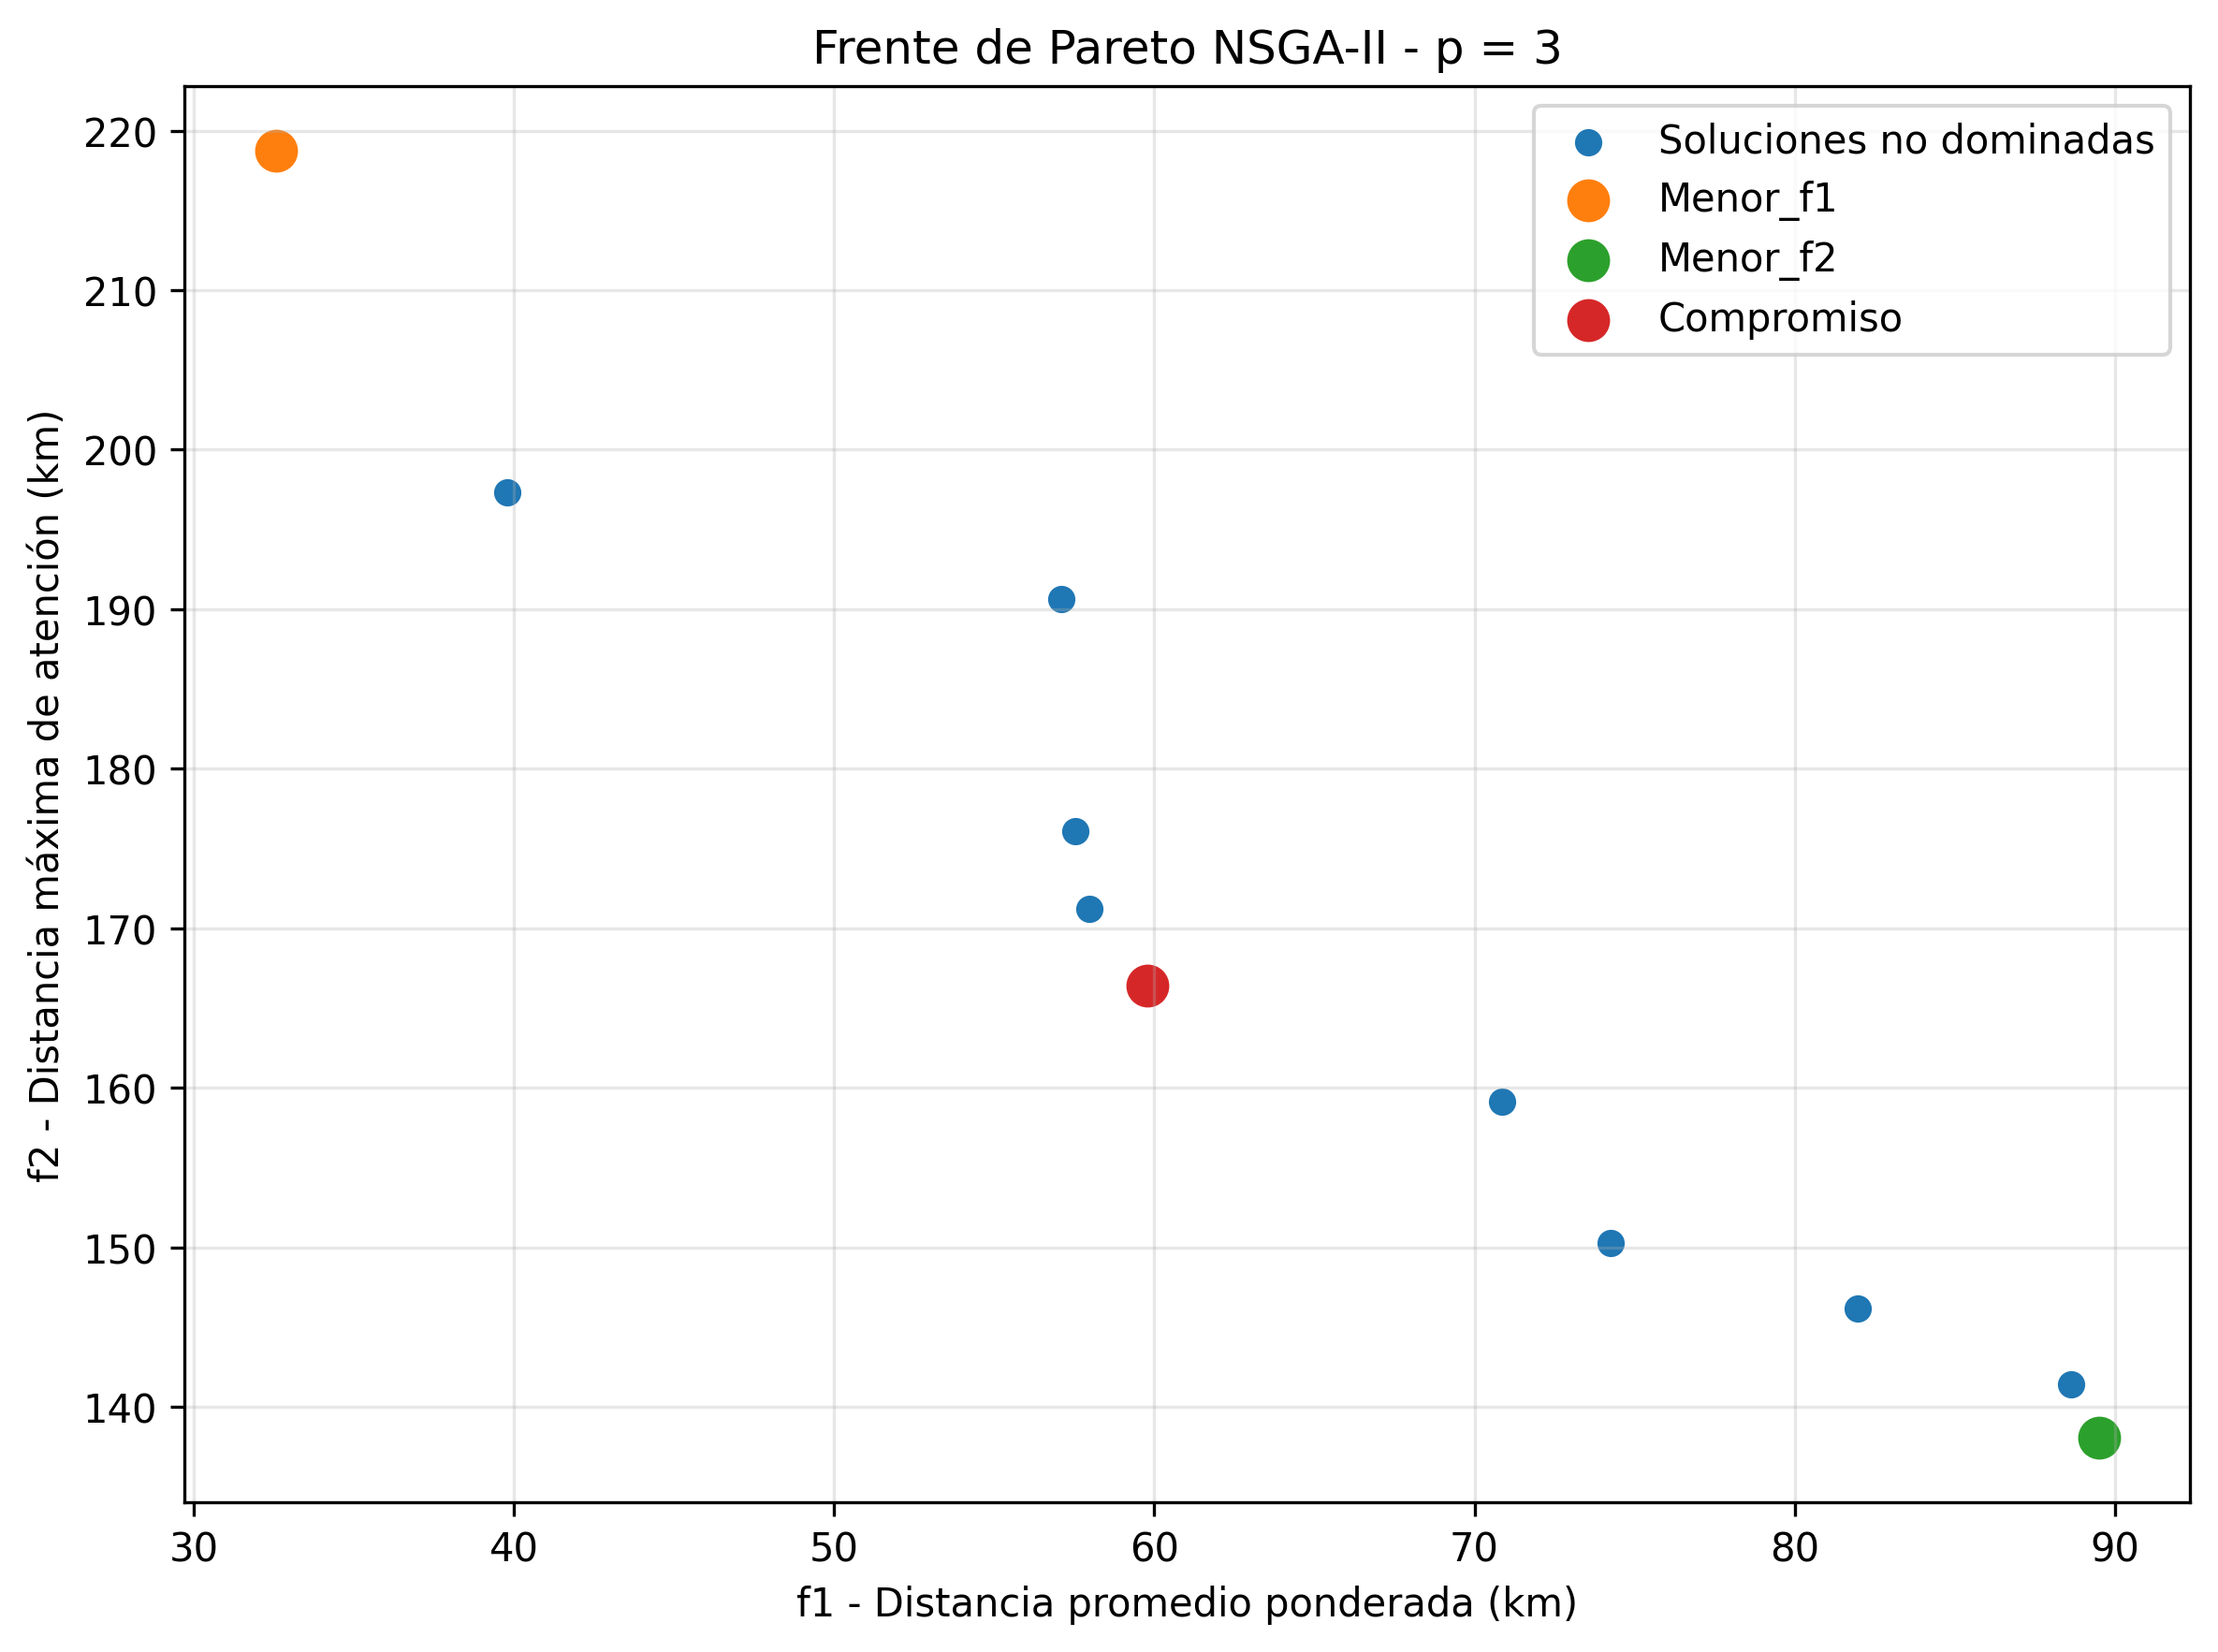
\includegraphics[width=0.75\linewidth]{frente_pareto_p3.png}
	\caption{Frente de Pareto obtenido mediante NSGA-II para $p=3$.}
	\label{fig:pareto_p3}
\end{figure}

\begin{figure}[!t]
	\centering
	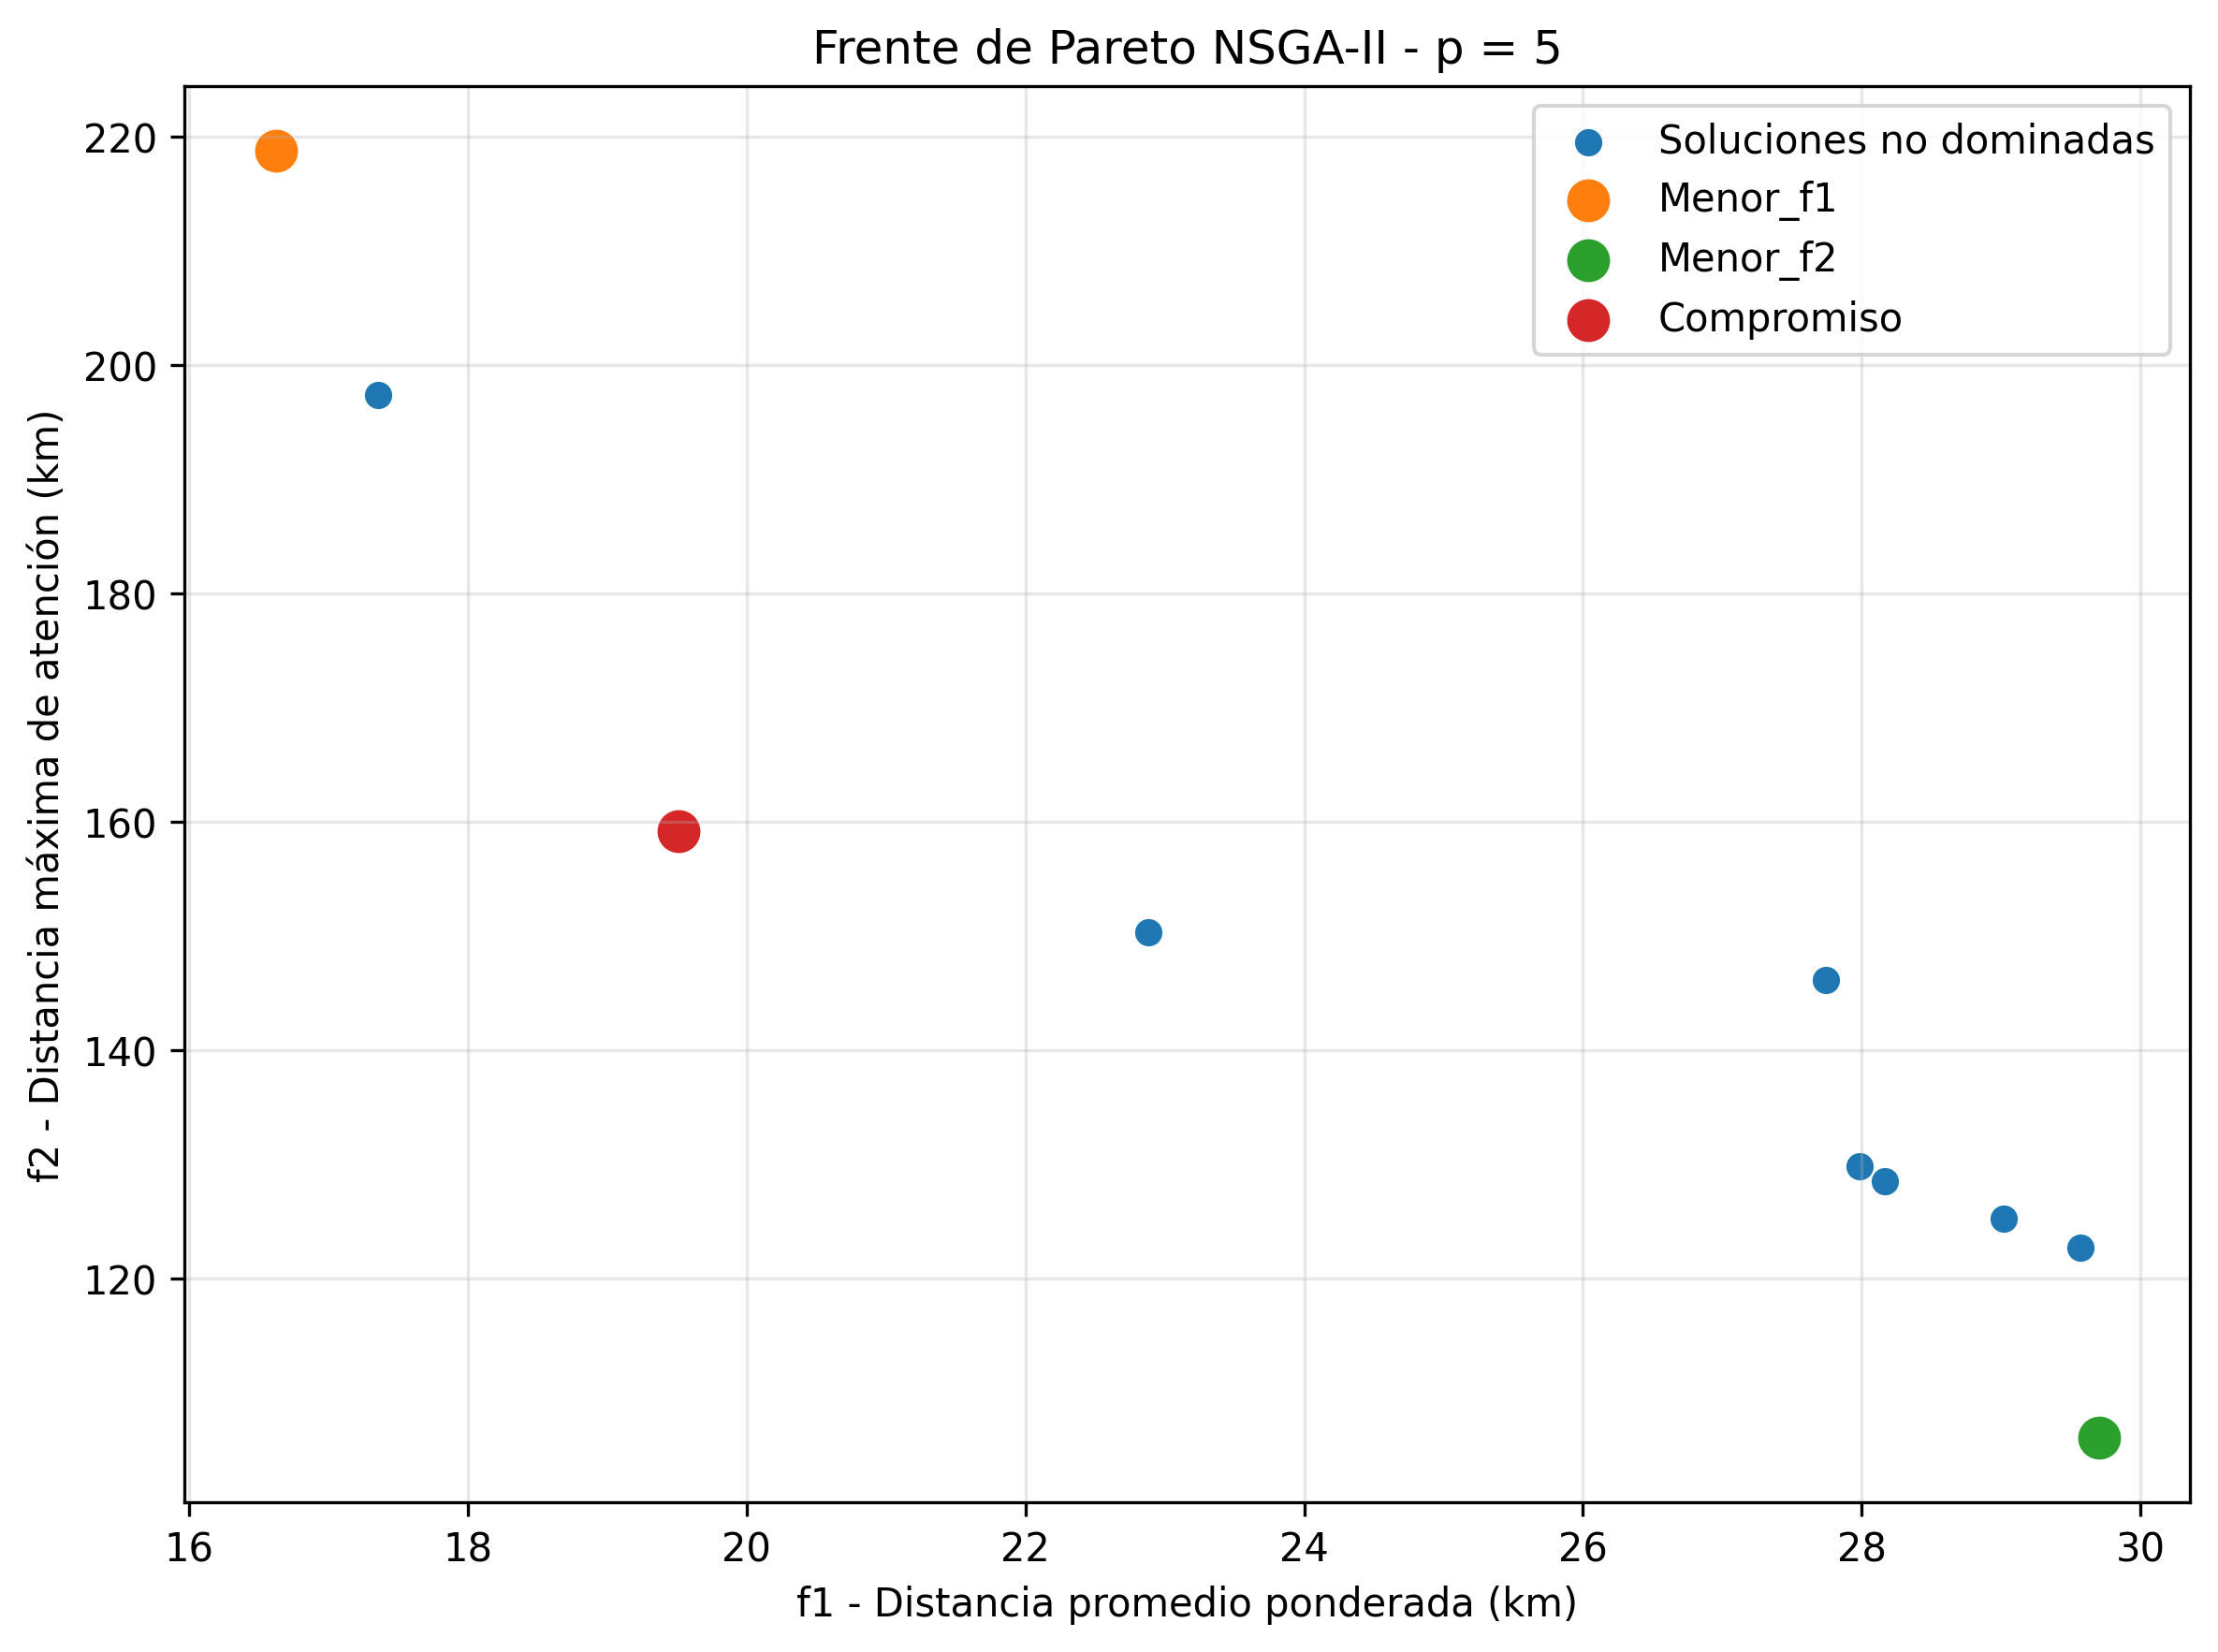
\includegraphics[width=0.75\linewidth]{frente_pareto_p5.png}
	\caption{Frente de Pareto obtenido mediante NSGA-II para $p=5$.}
	\label{fig:pareto_p5}
\end{figure}

\begin{figure}[!t]
	\centering
	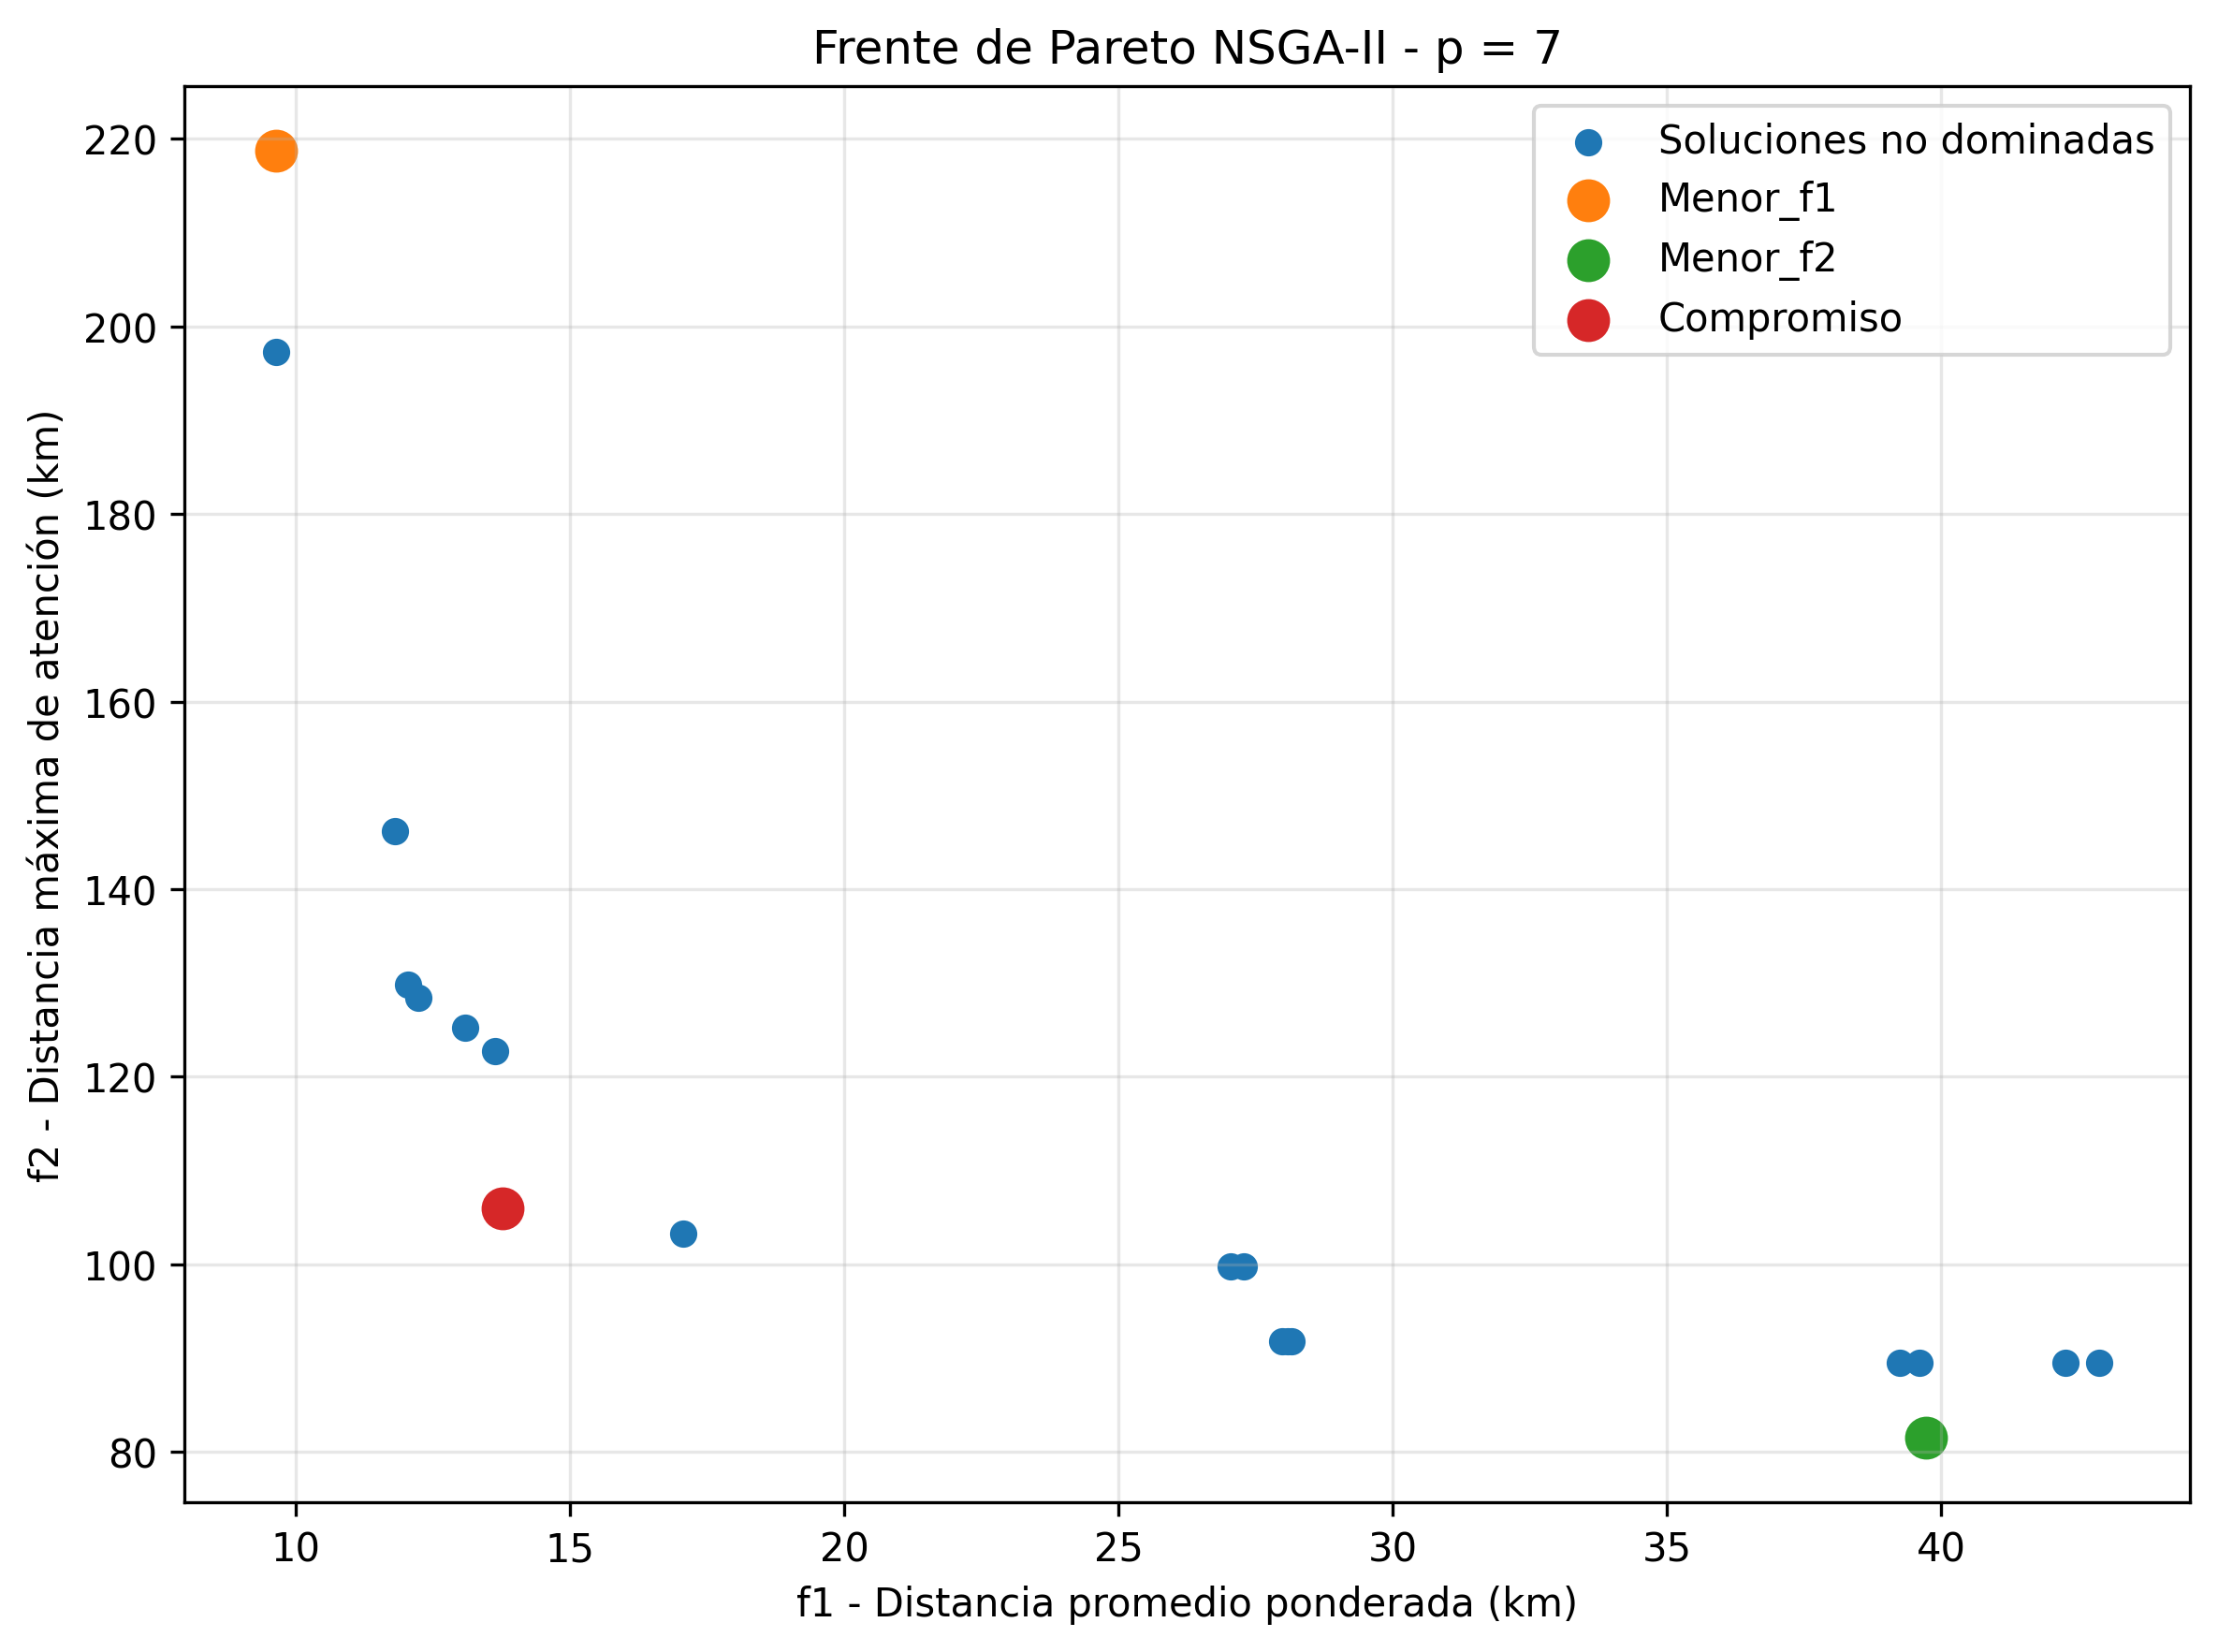
\includegraphics[width=0.75\linewidth]{frente_pareto_p7.png}
	\caption{Frente de Pareto obtenido mediante NSGA-II para $p=7$.}
	\label{fig:pareto_p7}
\end{figure}

\begin{figure}[!t]
	\centering
	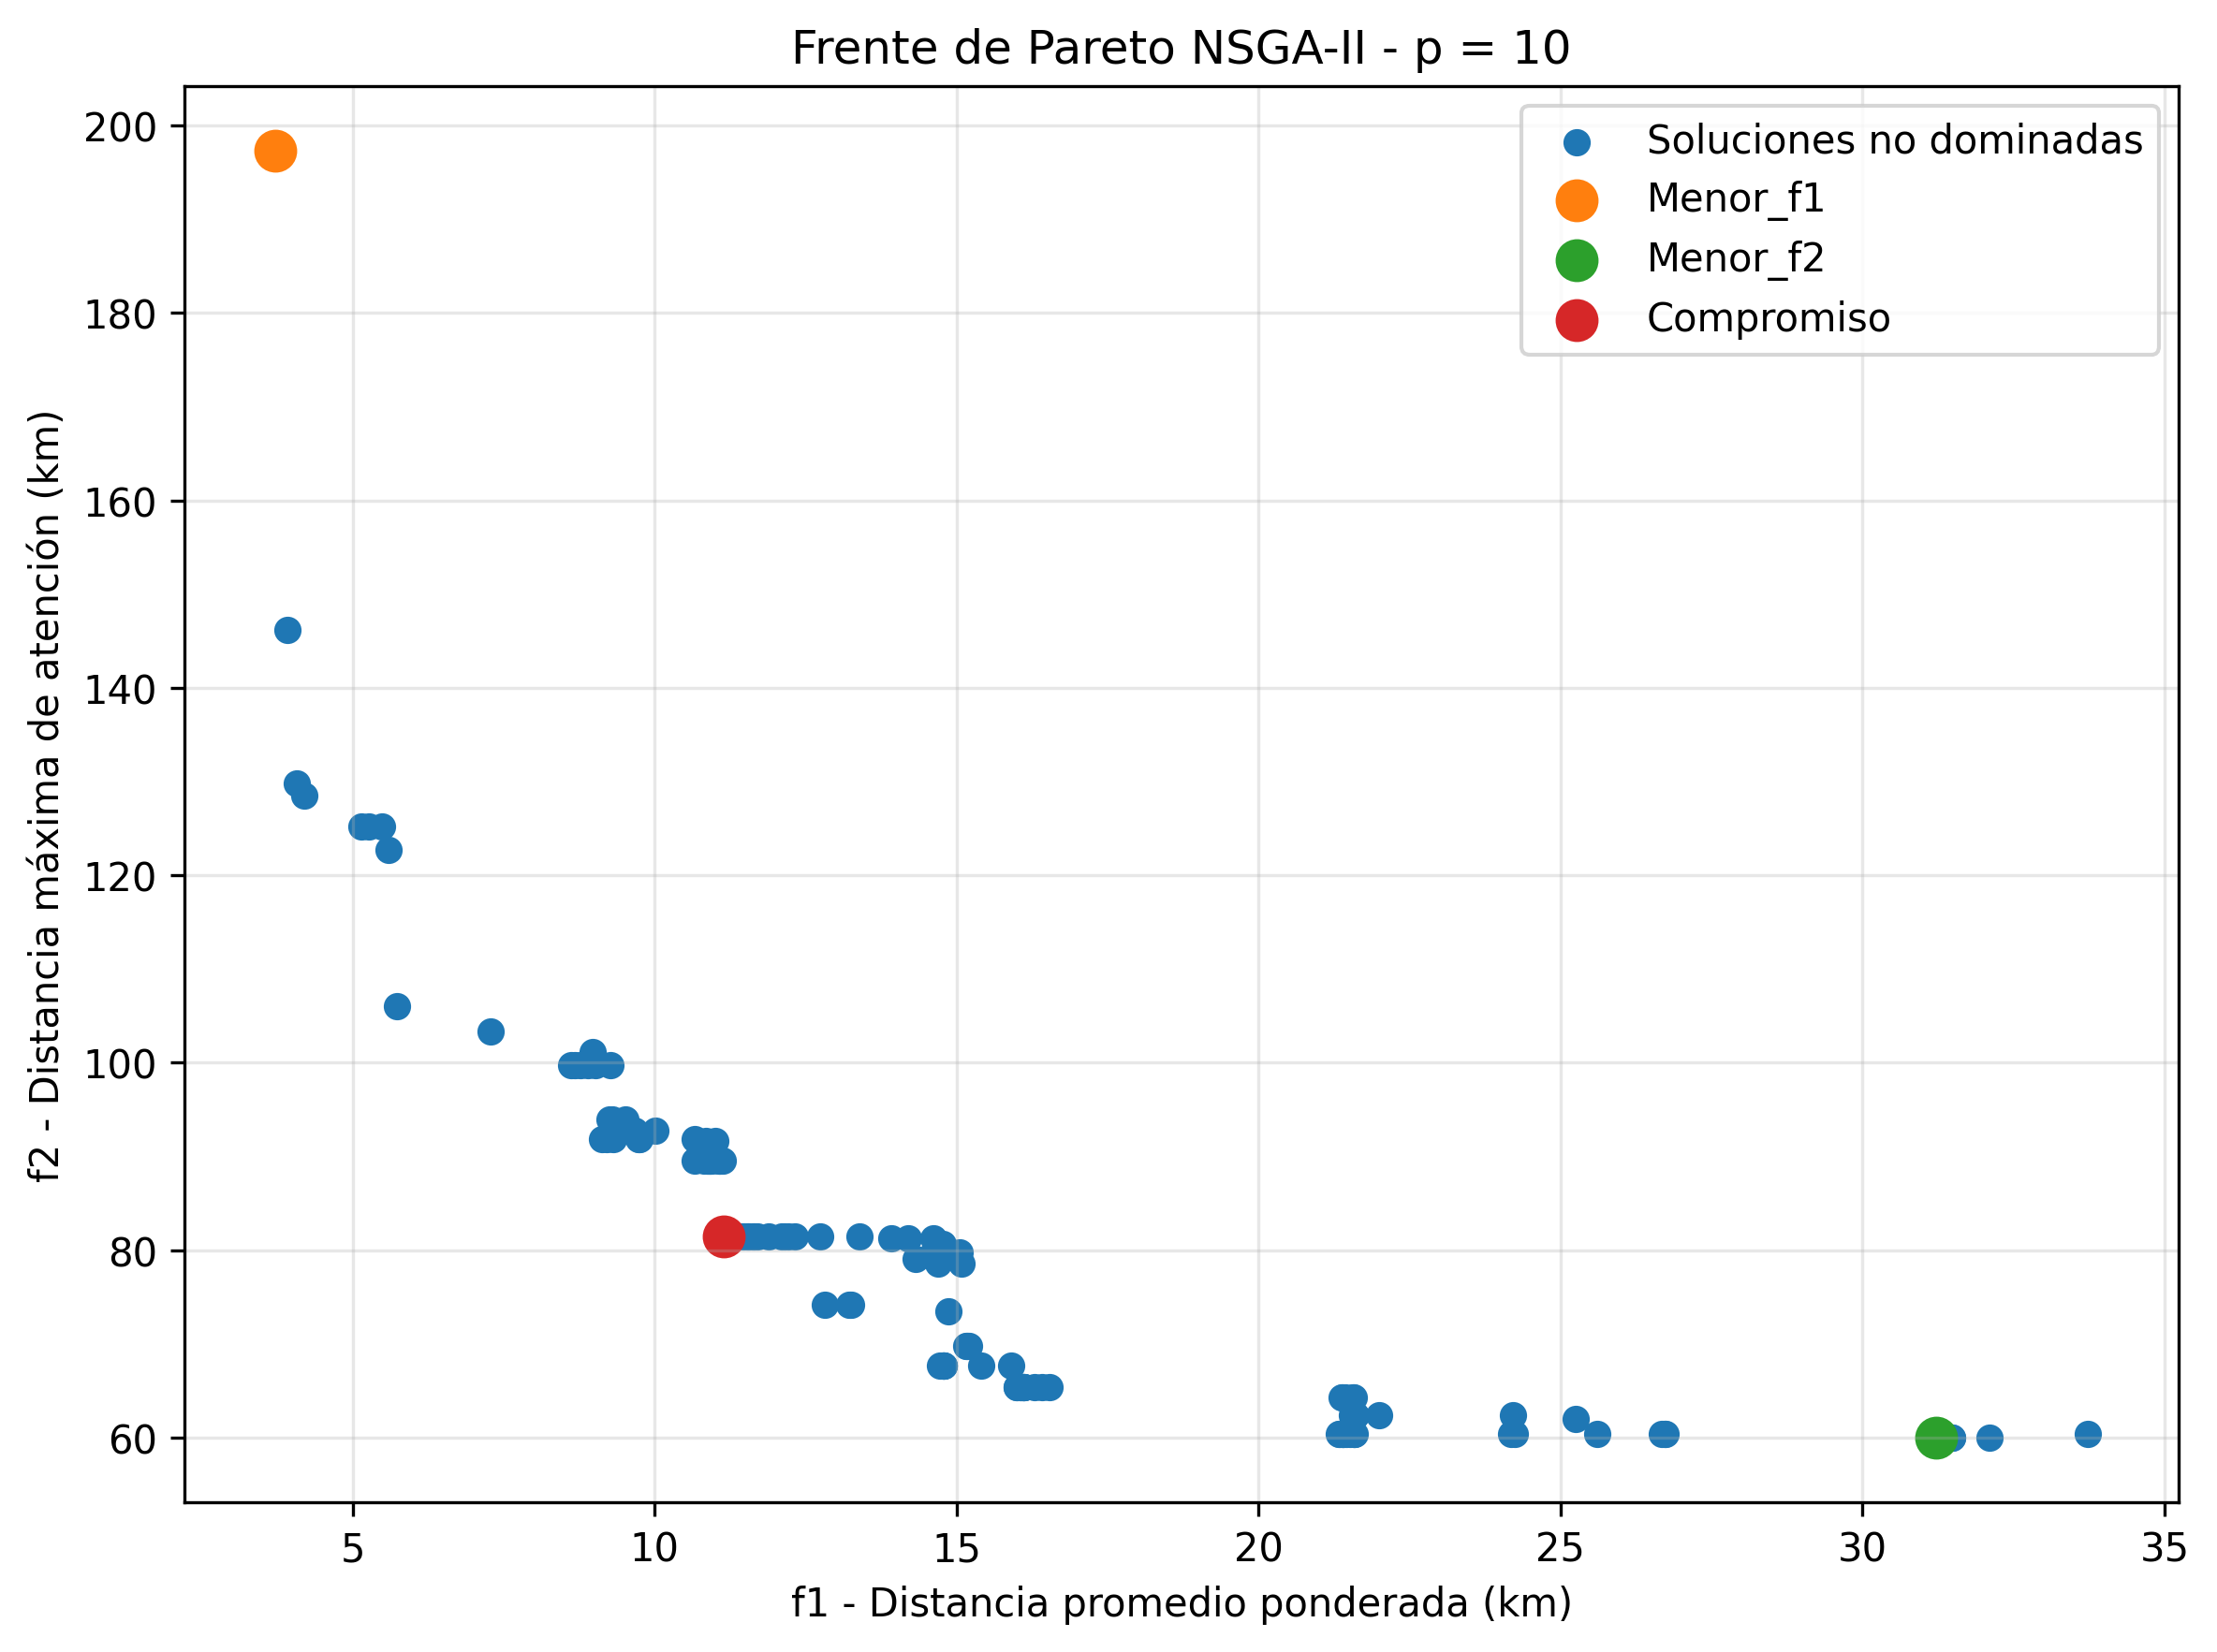
\includegraphics[width=0.75\linewidth]{frente_pareto_p10.png}
	\caption{Frente de Pareto obtenido mediante NSGA-II para $p=10$.}
	\label{fig:pareto_p10}
\end{figure}


Los frentes de Pareto obtenidos muestran que no existe una única solución que minimice simultáneamente ambos objetivos. Las soluciones ubicadas hacia valores bajos de $f_1$ favorecen la eficiencia en el traslado de la producción, mientras que aquellas con valores bajos de $f_2$ favorecen una distribución territorial más equilibrada de los centros de acopio.

A medida que aumenta $p$, los frentes se desplazan hacia regiones con menores valores de ambos objetivos, lo que indica una mejora general en la capacidad de atención. Sin embargo, incluso con un mayor número de centros continúa existiendo un intercambio entre minimizar la distancia promedio ponderada y reducir la máxima distancia de atención.

\subsection{Resultados de la optimización con tres objetivos}

La incorporación del número de centros como tercer objetivo permitió analizar el comportamiento de las soluciones cuando la cantidad de instalaciones dejó de fijarse previamente y pasó a formar parte del proceso de optimización. Las soluciones no dominadas obtenidas incluyeron configuraciones de entre 3 y 10 centros, cumpliendo en todos los casos la restricción establecida.

Para evaluar el efecto del número de instalaciones sobre el desempeño del sistema, se identificó, para cada configuración, el menor valor encontrado de la distancia promedio ponderada por producción, $f_1$, así como el menor valor de la distancia máxima de atención, $f_2$. Los resultados correspondientes se presentan en la Tabla~\ref{tab:resultados_tres_objetivos}.

\begin{table}[!t]
	\centering
	\caption{Mejores valores encontrados según el número de centros.}
	\label{tab:resultados_tres_objetivos}
	\begin{tabular}{ccccc}
		\toprule
		\textbf{Centros} &
		\textbf{Menor $f_1$} &
		\textbf{$f_2$ asociado} &
		\textbf{Menor $f_2$} &
		\textbf{$f_1$ asociado} \\
		& \textbf{(km)} & \textbf{(km)} & \textbf{(km)} & \textbf{(km)} \\
		\midrule
		3  & 32.5614 & 218.7570 & 138.0459 & 89.5045 \\
		4  & 20.4873 & 218.7570 & 125.2327 & 54.2841 \\
		5  & 16.6217 & 218.7570 & 106.0083 & 29.7023 \\
		6  & 12.7804 & 218.7570 & 95.2291  & 41.3434 \\
		7  & 9.6398  & 218.7570 & 81.4828  & 39.8122 \\
		8  & 6.5049  & 197.3279 & 77.8516  & 42.7399 \\
		9  & 4.5419  & 197.3279 & 64.3055  & 33.4717 \\
		10 & 3.7921  & 197.3279 & 64.3055  & 21.3976 \\
		\bottomrule
	\end{tabular}
\end{table}

El menor valor de $f_1$ disminuyó progresivamente conforme aumentó el número de centros. Con tres instalaciones se obtuvo una distancia promedio ponderada mínima de 32.5614 km, mientras que con diez centros este valor se redujo a 3.7921 km. Este comportamiento muestra que el incremento en el número de instalaciones favorece la reducción de las distancias de traslado, principalmente para los municipios con mayor producción agrícola.

Sin embargo, las soluciones orientadas a minimizar $f_1$ no necesariamente proporcionaron una mejor cobertura territorial. Para configuraciones de entre tres y siete centros, las soluciones con menor $f_1$ presentaron una distancia máxima de atención de 218.7570 km. Esto evidencia el conflicto entre ambos objetivos, ya que reducir la distancia promedio ponderada puede mantener algunos municipios a distancias considerablemente mayores de su centro de acopio más cercano.

Por otra parte, el menor valor de $f_2$ disminuyó de 138.0459 km con tres centros a 64.3055 km con nueve centros, mostrando una mejora progresiva en la cobertura territorial conforme se incorporaron nuevas instalaciones. Al aumentar de nueve a diez centros, el menor valor encontrado de $f_2$ permaneció en 64.3055 km. Por lo tanto, dentro de las soluciones obtenidas, la incorporación de una décima instalación no produjo una mejora adicional en la distancia máxima de atención.

\begin{figure}[!t]
	\centering
	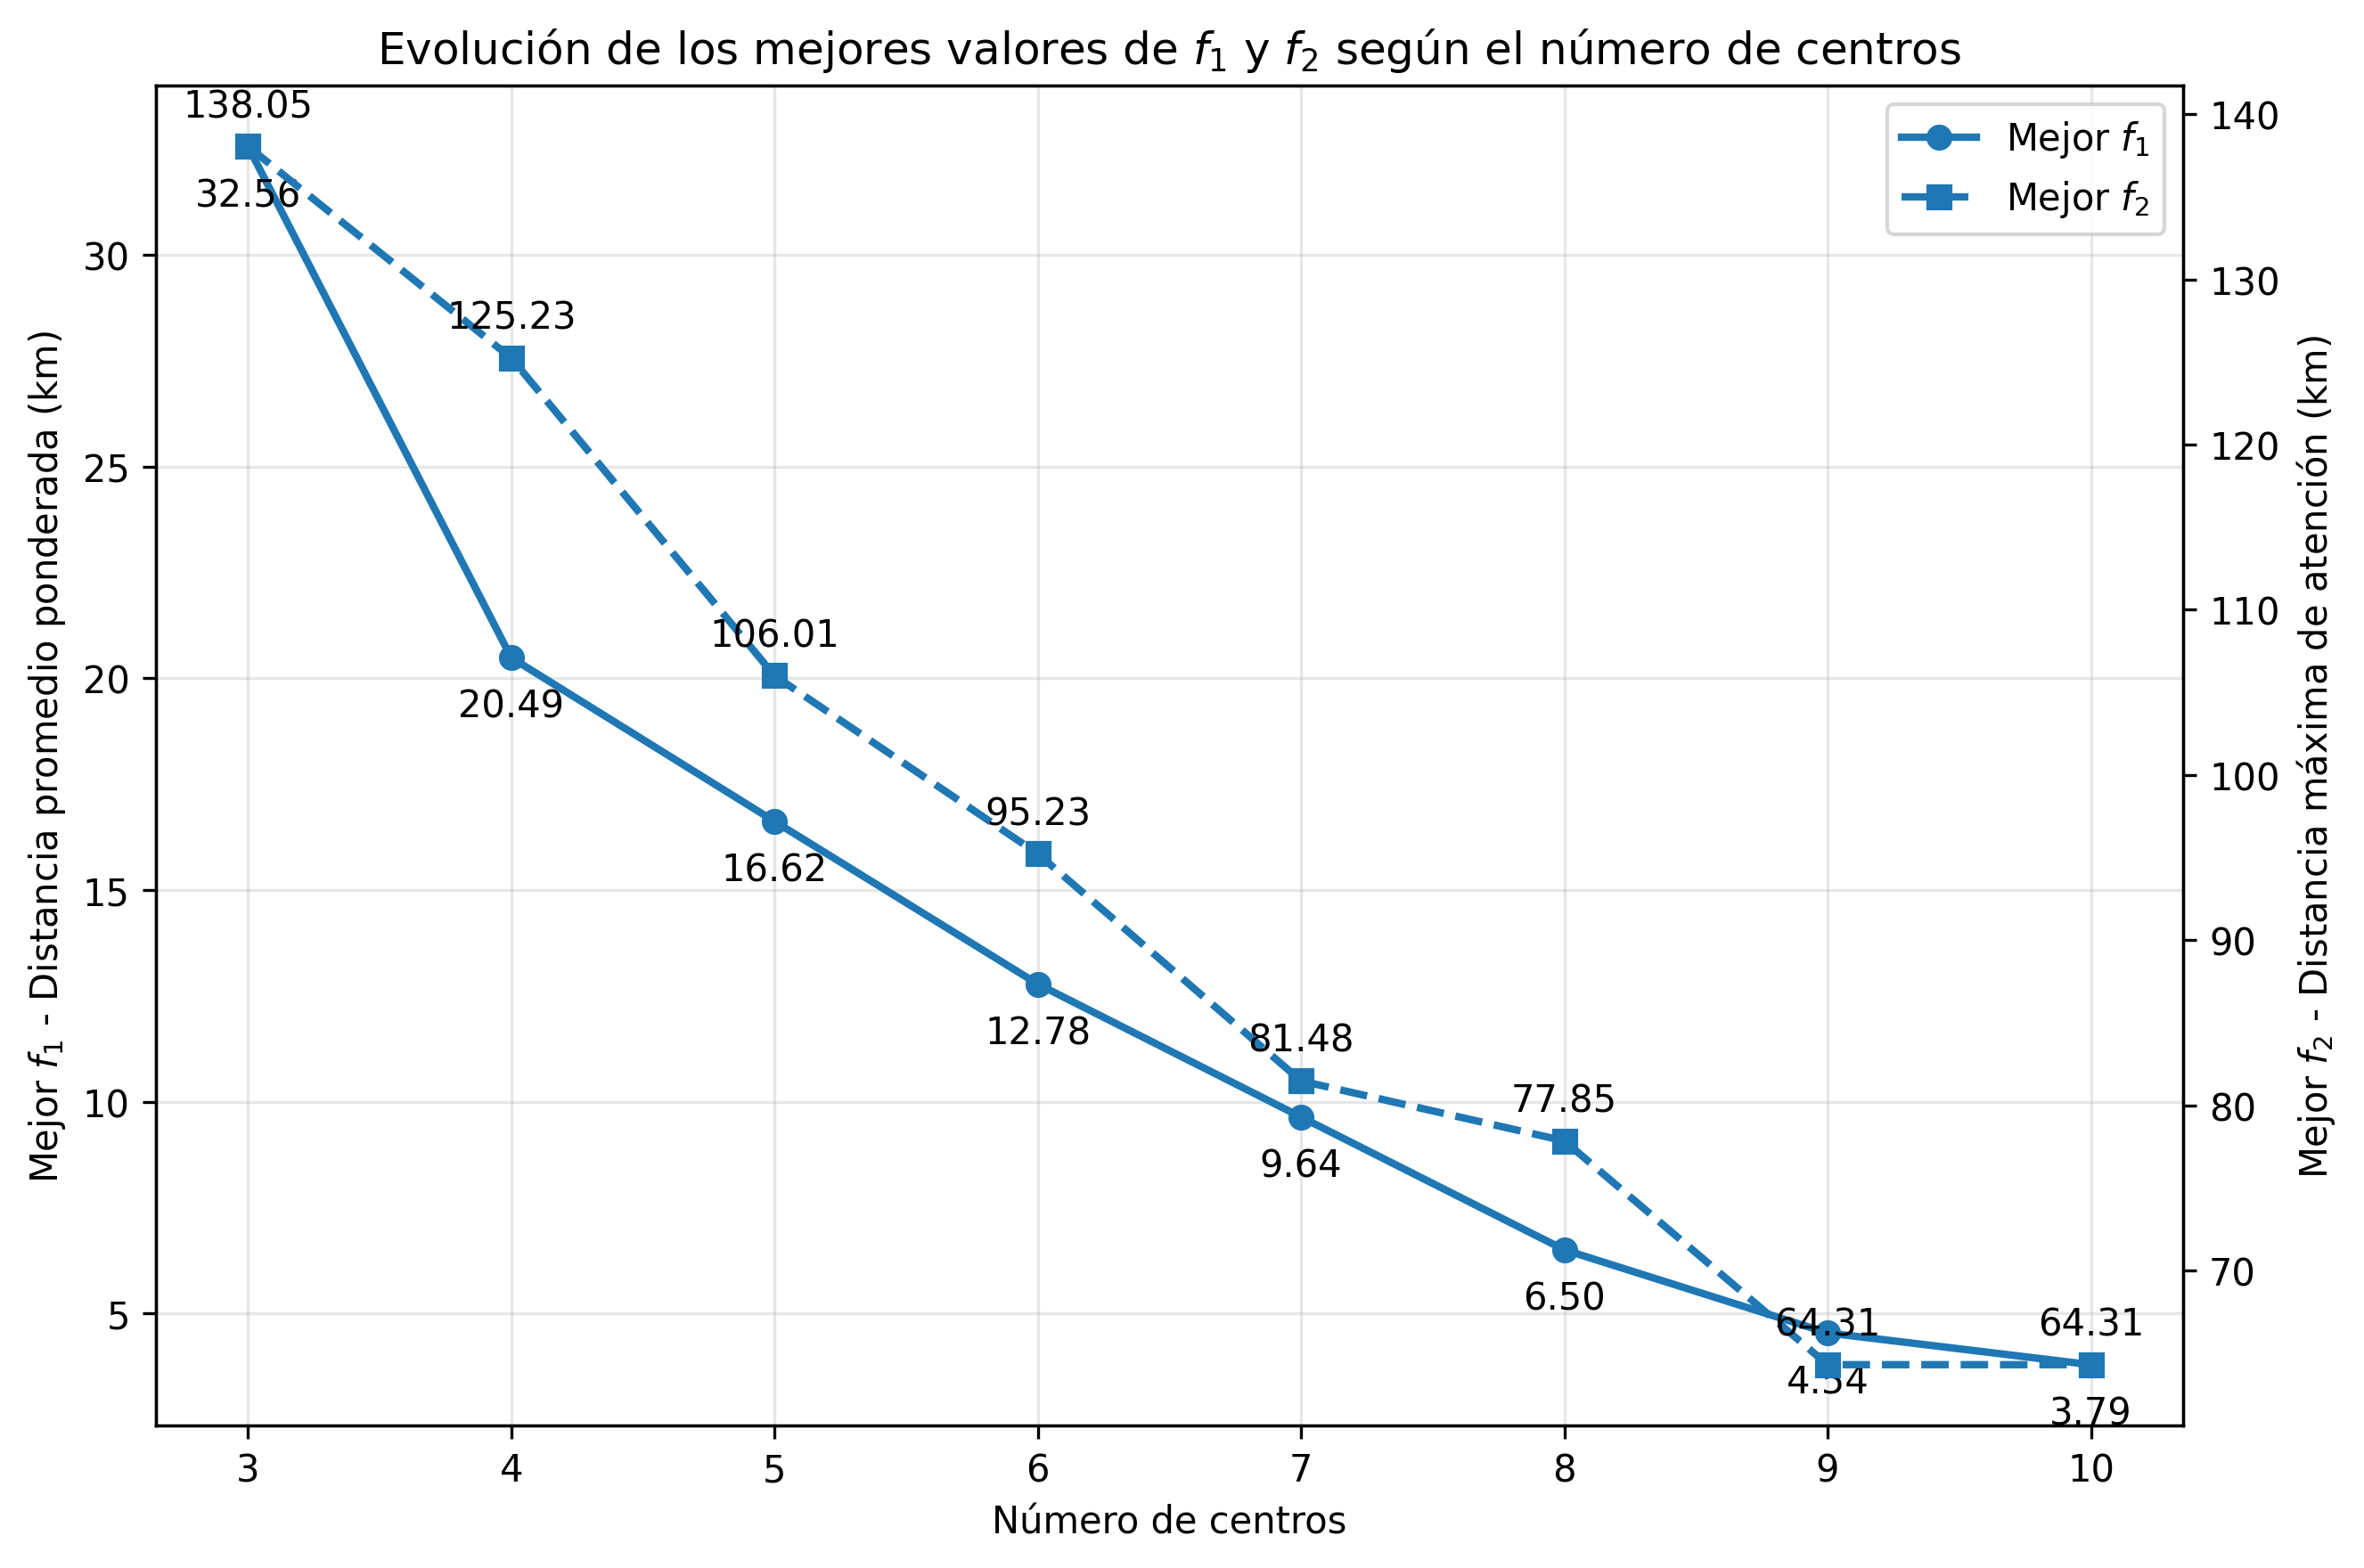
\includegraphics[width=0.85\linewidth]
	{evolucion_f1_f2_numero_centros.png}
	\caption{Evolución de los mejores valores de $f_1$ y $f_2$ en función del número de centros de acopio.}
	\label{fig:evolucion_tres_objetivos}
\end{figure}

Como se observa en la Figura~\ref{fig:evolucion_tres_objetivos}, ambos criterios presentan una tendencia general de mejora conforme aumenta el número de instalaciones. Sin embargo, la magnitud de esta mejora varía entre configuraciones consecutivas, lo que permite analizar el beneficio obtenido al incorporar un centro adicional y determinar en qué punto dicho beneficio comienza a disminuir.

Los mejores valores obtenidos en esta formulación no necesariamente coinciden con los alcanzados en los experimentos anteriores con un número fijo de centros. Esto se debe a que la incorporación de $f_3$ modifica el problema de optimización, ya que NSGA-II debe evaluar simultáneamente soluciones con diferentes cantidades de instalaciones y establecer compromisos entre los tres objetivos. Por ejemplo, para diez centros se obtuvo un valor mínimo de $f_1=3.7921$ km en la formulación de tres objetivos, mientras que en la formulación con un número fijo de centros se alcanzó $f_1=3.7218$ km. Esta diferencia refleja el efecto de incorporar el número de instalaciones como un objetivo adicional dentro del proceso de optimización.

\subsubsection{Análisis marginal del número de centros}

El análisis marginal permitió cuantificar el beneficio obtenido al incrementar en una unidad el número de centros de acopio. La mayor reducción absoluta de $f_1$ se presentó al pasar de tres a cuatro centros, con una disminución de 12.0741 km, equivalente al 37.08\% respecto a la configuración anterior. A partir de este punto, las reducciones absolutas fueron menores, aunque la distancia promedio ponderada continuó disminuyendo hasta alcanzar su menor valor con diez centros.

Para $f_2$, las mejoras presentaron un comportamiento menos uniforme. Al pasar de ocho a nueve centros se obtuvo una reducción de 13.5461 km, equivalente al 17.40\%. Sin embargo, la incorporación de un décimo centro no produjo una reducción adicional, por lo que el menor valor encontrado de la distancia máxima de atención se mantuvo en 64.3055 km.

Estos resultados muestran que incrementar el número de instalaciones no produce necesariamente una mejora proporcional en todos los objetivos. La configuración de nueve centros resulta relevante desde la perspectiva de cobertura territorial, debido a que agregar una décima instalación no redujo el menor valor encontrado de $f_2$. No obstante, esta última incorporación sí permitió disminuir $f_1$ de 4.5419 km a 3.7921 km. Por lo tanto, la conveniencia de aumentar el número de centros depende del compromiso establecido entre la reducción de la distancia promedio ponderada, la cobertura territorial y la cantidad de infraestructura requerida.

\section{Discusión}

\subsection{Comparación entre las líneas base y el algoritmo genético}

Las líneas base permitieron establecer puntos de referencia para evaluar el desempeño del algoritmo genético. La selección aleatoria presentó los mayores valores de distancia promedio ponderada en todas las configuraciones analizadas, mientras que las estrategias basadas en producción y selección voraz proporcionaron soluciones considerablemente mejores. Esto evidencia la importancia de considerar información relacionada con la producción y las distancias entre municipios durante la selección de los centros de acopio.

Para $p=3$, el algoritmo genético obtuvo una distancia promedio ponderada de 32.5614 km, mejorando los 38.9035 km obtenidos mediante la estrategia basada en producción y los 38.0230 km de la estrategia voraz. Para $p=5$, el algoritmo genético alcanzó un valor de 16.6217 km, igualando el resultado de la estrategia voraz y superando los 31.9029 km obtenidos mediante la selección basada en producción.

Un comportamiento similar se observó para $p=7$ y $p=10$, donde el algoritmo genético alcanzó distancias promedio ponderadas de 9.6398 km y 3.7218 km, respectivamente, coincidiendo con los mejores valores obtenidos mediante la estrategia voraz. Por lo tanto, el algoritmo genético no superó a esta heurística en todas las configuraciones evaluadas; sin embargo, logró igualar o mejorar sus resultados para todos los valores de $p$, mostrando un desempeño consistente en la búsqueda de configuraciones con menores distancias promedio ponderadas.

Las diferencias fueron más evidentes al comparar el algoritmo genético con la selección aleatoria. Las reducciones de la distancia promedio ponderada fueron de 72.91\%, 78.81\%, 86.97\% y 92.36\% para $p=3$, $p=5$, $p=7$ y $p=10$, respectivamente. La prueba de Wilcoxon obtuvo un valor de $p=1.862645\times10^{-9}$ para las cuatro configuraciones, inferior al nivel de significancia de 0.05. Por lo tanto, se identificaron diferencias estadísticamente significativas entre los resultados del algoritmo genético y los obtenidos mediante la selección aleatoria.

\subsection{Estabilidad del algoritmo genético}

Las 30 corridas independientes del algoritmo genético convergieron al mismo valor de la función objetivo y a la misma configuración de centros para cada valor de $p$. Como resultado, la desviación estándar del fitness fue igual a cero en los cuatro escenarios evaluados, lo que evidencia una alta consistencia de los resultados bajo las condiciones experimentales establecidas.

Además, para $p=5$, $p=7$ y $p=10$, el algoritmo genético alcanzó los mismos valores de la función objetivo que la estrategia voraz, mientras que para $p=3$ obtuvo un resultado superior. Estos resultados indican que el algoritmo genético fue capaz de encontrar de manera consistente configuraciones favorables para minimizar la distancia promedio ponderada.

Sin embargo, la ausencia de variabilidad entre las 30 corridas no constituye una demostración de optimalidad global. Debido a que no se realizó una evaluación exhaustiva de todas las combinaciones posibles de centros, los resultados deben interpretarse como evidencia de estabilidad y reproducibilidad del algoritmo bajo la configuración experimental utilizada.

\subsection{Comparación entre GA y NSGA-II}

El algoritmo genético monoobjetivo y NSGA-II responden a diferentes criterios de optimización. Mientras que el GA busca una única configuración orientada a minimizar la distancia promedio ponderada por producción, NSGA-II permite obtener un conjunto de soluciones no dominadas que representan distintos compromisos entre eficiencia logística y cobertura territorial.

Los resultados muestran que las soluciones de NSGA-II orientadas a minimizar $f_1$ alcanzan valores iguales o cercanos a los obtenidos mediante el algoritmo genético monoobjetivo. Sin embargo, una solución favorable para este criterio puede presentar una distancia máxima de atención elevada. Por ejemplo, para $p=3$, la solución con $f_1=32.5614$ km presentó un valor de $f_2=218.7570$ km, lo que indica que algunos municipios permanecen considerablemente alejados de su centro de acopio más cercano.

Al considerar simultáneamente ambos objetivos, NSGA-II permitió identificar alternativas con una mejor cobertura territorial a cambio de incrementar la distancia promedio ponderada. Para $p=3$, la menor distancia máxima de atención encontrada fue de 138.0459 km, mientras que $f_1$ aumentó a 89.5045 km. Este comportamiento evidencia el conflicto existente entre ambos objetivos y muestra que minimizar únicamente la distancia promedio ponderada puede favorecer a los municipios con mayor producción sin garantizar una cobertura territorial equilibrada.

\subsection{Número de centros de acopio}

La formulación con tres objetivos permitió incorporar el número de centros de acopio como parte del proceso de optimización. En términos generales, el incremento en la cantidad de instalaciones produjo una reducción en las distancias de atención. Sin embargo, la magnitud de las mejoras obtenidas varió entre las diferentes configuraciones evaluadas.

La menor distancia promedio ponderada disminuyó de 32.5614 km con tres centros a 4.5419 km con nueve centros. De manera similar, la menor distancia máxima de atención se redujo de 138.0459 km a 64.3055 km en el mismo intervalo, mostrando que el aumento en el número de instalaciones favoreció tanto la eficiencia promedio como la cobertura territorial.

Al incrementar la configuración de nueve a diez centros, el menor valor encontrado de $f_2$ permaneció en 64.3055 km. En contraste, $f_1$ continuó disminuyendo, pasando de 4.5419 km a 3.7921 km. Esto indica que la incorporación de un décimo centro permitió mejorar la distancia promedio ponderada, pero no produjo una reducción adicional en la menor distancia máxima de atención encontrada.

Bajo los criterios considerados, la configuración de nueve centros representa una alternativa relevante de compromiso, ya que permitió alcanzar el menor valor observado de $f_2$ sin utilizar el número máximo de instalaciones permitido. Sin embargo, estos resultados no permiten establecer nueve centros como una configuración óptima definitiva. Para determinar el número de instalaciones más conveniente en una aplicación real sería necesario incorporar criterios adicionales, como costos de instalación y operación, capacidad de los centros, infraestructura disponible y restricciones presupuestarias.

\subsection{Efecto de incorporar el número de centros como objetivo}

La incorporación de $f_3$ modificó la formulación del problema, debido a que el número de centros dejó de establecerse previamente y pasó a formar parte de los criterios considerados durante la optimización. En la formulación de dos objetivos fue necesario evaluar de manera independiente las configuraciones con $p=3$, $p=5$, $p=7$ y $p=10$. En cambio, la formulación con tres objetivos permitió explorar, dentro de un mismo proceso evolutivo, soluciones con entre 3 y 10 instalaciones.

Este enfoque permite analizar de manera conjunta el beneficio logístico asociado con el incremento de la infraestructura. Los resultados mostraron que aumentar el número de centros tiende a reducir tanto la distancia promedio ponderada, $f_1$, como la distancia máxima de atención, $f_2$. Sin embargo, esta mejora implica un incremento en $f_3$, correspondiente al número de instalaciones requeridas. De esta manera, los tres objetivos presentan un compromiso que debe considerarse de forma conjunta durante la selección de una solución.

La formulación de tres objetivos proporciona un conjunto de alternativas con diferentes niveles de eficiencia logística, cobertura territorial y cantidad de infraestructura, sin establecer previamente un número fijo de centros. Esto permite que la selección final de una configuración se realice en función de las prioridades del problema y del balance deseado entre los tres criterios considerados.

\section{Conclusiones}

En este proyecto se abordó el problema de localización de centros de acopio agrícola en Tamaulipas mediante técnicas de cómputo evolutivo, considerando la producción agrícola de los 43 municipios y las distancias entre sus cabeceras municipales. La implementación de líneas base, un algoritmo genético monoobjetivo y NSGA-II permitió evaluar diferentes estrategias de optimización y analizar el comportamiento de las soluciones bajo distintos criterios.

El algoritmo genético presentó un desempeño superior a la selección aleatoria para todos los valores de $p$ evaluados, con reducciones de la distancia promedio ponderada de 72.91%, 78.81%, 86.97% y 92.36% para $p=3$, $p=5$, $p=7$ y $p=10$, respectivamente. Estas diferencias resultaron estadísticamente significativas de acuerdo con la prueba de Wilcoxon. Asimismo, el algoritmo genético superó a la estrategia voraz para $p=3$ e igualó sus resultados para $p=5$, $p=7$ y $p=10$, mostrando que ambas estrategias fueron capaces de obtener soluciones competitivas para la formulación monoobjetivo considerada.

La formulación multiobjetivo mediante NSGA-II permitió evidenciar que minimizar únicamente la distancia promedio ponderada no garantiza una cobertura territorial equilibrada. Algunas de las soluciones con menores valores de $f_1$ presentaron distancias máximas de atención elevadas. Al considerar simultáneamente $f_1$ y $f_2$, los frentes de Pareto permitieron identificar diferentes compromisos entre eficiencia logística y cobertura territorial, proporcionando un conjunto de alternativas en lugar de una única configuración.

La incorporación del número de centros como tercer objetivo permitió analizar conjuntamente la eficiencia logística, la cobertura territorial y la cantidad de infraestructura requerida. Los resultados mostraron una reducción general de las distancias conforme aumentó el número de instalaciones, aunque los beneficios adicionales no fueron uniformes. En particular, con nueve centros se alcanzó el menor valor encontrado de la distancia máxima de atención, correspondiente a 64.3055 km, sin observar una reducción adicional al incorporar un décimo centro. En contraste, la distancia promedio ponderada continuó disminuyendo de 4.5419 km con nueve centros a 3.7921 km con diez centros.

Bajo las condiciones y objetivos considerados, la configuración de nueve centros representa una alternativa relevante de compromiso, ya que permitió alcanzar la menor distancia máxima encontrada sin utilizar el número máximo de instalaciones permitido. Sin embargo, este resultado no debe interpretarse como una configuración óptima definitiva, debido a que el modelo no considera factores como costos de construcción y operación, capacidades de almacenamiento, infraestructura carretera o restricciones presupuestarias.

En conjunto, los resultados muestran que el cómputo evolutivo constituye una herramienta adecuada para explorar problemas de localización con múltiples criterios en conflicto. Mientras que la optimización monoobjetivo permitió identificar configuraciones favorables para reducir la distancia promedio ponderada, la optimización multiobjetivo proporcionó una visión más amplia de las alternativas disponibles y de los compromisos asociados con cada decisión. Como trabajo futuro, incorporar costos, capacidades y restricciones logísticas permitiría extender el modelo hacia un escenario más representativo de la planificación de centros de acopio agrícola en Tamaulipas.



\begin{thebibliography}{1}
	
	\bibitem{blank2020pymoo}
	J. Blank and K. Deb,
	``pymoo: Multi-Objective Optimization in Python,''
	\textit{IEEE Access},
	vol. 8, pp. 89497--89509, 2020,
	doi: 10.1109/ACCESS.2020.2990567.
	
	\bibitem{eiben2015introduction}
	A. E. Eiben and J. E. Smith,
	\textit{Introduction to Evolutionary Computing},
	2nd ed.
	Berlin, Heidelberg: Springer, 2015,
	doi: 10.1007/978-3-662-44874-8.
	
	\bibitem{mladenovic2007pmedian}
	N. Mladenovi\'c, J. Brimberg, P. Hansen, and J. A. Moreno-P\'erez,
	``The $p$-median problem: A survey of metaheuristic approaches,''
	\textit{European Journal of Operational Research},
	vol. 179, no. 3, pp. 927--939, 2007,
	doi: 10.1016/j.ejor.2005.05.034.
	
	\bibitem{farahani2010facility}
	R. Z. Farahani, M. SteadieSeifi, and N. Asgari,
	``Multiple criteria facility location problems: A survey,''
	\textit{Applied Mathematical Modelling},
	vol. 34, no. 7, pp. 1689--1709, 2010.
	
	\bibitem{deb2002nsga2}
	K. Deb, A. Pratap, S. Agarwal, and T. Meyarivan,
	``A fast and elitist multiobjective genetic algorithm: NSGA-II,''
	\textit{IEEE Transactions on Evolutionary Computation},
	vol. 6, no. 2, pp. 182--197, 2002,
	doi: 10.1109/4235.996017.
	

\end{thebibliography}


\end{document}


